%% Copyright 2019-2024 Elsevier Ltd
%%
%% This file is part of the 'CAS Bundle'.
%% --------------------------------------
%%
%% It may be distributed under the conditions of the LaTeX Project Public
%% License, either version 1.3c of this license or (at your option) any
%% later version.  The latest version of this license is in
%%    http://www.latex-project.org/lppl.txt
%% and version 1.3c or later is part of all distributions of LaTeX
%% version 1999/12/01 or later.
%%
%% The list of all files belonging to the 'CAS Bundle' is
%% given in the file `manifest.txt'.
%%
%% Template article for cas-dc documentclass for
%% double column output.
\documentclass[a4paper,fleqn]{cas-sc}
\usepackage{booktabs}
\usepackage{amsmath,amssymb}
\usepackage{graphicx}
\usepackage{xcolor}
\usepackage{pgfplots}
\pgfplotsset{compat=1.17}
\usetikzlibrary{arrows.meta,positioning,fit,backgrounds,calc}
\usepackage{caption}
\captionsetup{font=small,labelfont=bf}
\usepackage{enumitem}
\usepackage{url}
% If the frontmatter runs over more than one page
% use the longmktitle option.
%\documentclass[a4paper,fleqn,longmktitle]{cas-dc}
%\usepackage[numbers]{natbib}
%\usepackage[authoryear]{natbib}
\usepackage[authoryear,longnamesfirst]{natbib}
%%%Author macros
\def\tsc#1{\csdef{#1}{\textsc{\lowercase{#1}}\xspace}}
\tsc{WGM}
\tsc{QE}
%%%
% Uncomment and use as if needed
%\newtheorem{theorem}{Theorem}
%\newtheorem{lemma}[theorem]{Lemma}
%\newdefinition{rmk}{Remark}
%\newproof{pf}{Proof}
%\newproof{pot}{Proof of Theorem \ref{thm}}
\begin{document}
\let\WriteBookmarks\relax
\def\floatpagepagefraction{1}
\def\textpagefraction{.001}
% Short title
\shorttitle{Is Progress on the TOP Benchmark Measurable?}
% Short author
\shortauthors{Çetiner and Adebayo}
% Main title of the paper
\title [mode = title]{Is Progress on the TOP Benchmark Measurable? A Forensic Re-evaluation of HINT and MEXA-CTP}
% Title footnote mark
% \tnotemark[1]
% Title footnote 1.
% \tnotetext[1]{Title footnote text}
% First author
% \author[1,3]{Author Name}[type=editor,
%       style=chinese,
%       auid=000,
%       bioid=1,
%       prefix=Sir,
%       orcid=0000-0000-0000-0000,
%       facebook=<facebook id>,
%       twitter=<twitter id>,
%       linkedin=<linkedin id>,
%       gplus=<gplus id>]
\author[1]{Aziz Muammer Çetiner}[type=editor,
           orcid=0000-0000-0000-0000,]
% Footnote of the first author
%\fnmark[1]
% Email id of the first author
\ead{cetiner.aziz1@gmail.com}
% URL of the first author
%\ead[url]{}
% Credit authorship
% eg: \credit{Conceptualization of this study, Methodology, Software}
% Address/affiliation
\affiliation[1]{organization={},
            addressline={},
            city={},
%          citysep={}, % Uncomment if no comma needed between city and postcode
            postcode={},
            state={},
            country={}}
\author[2]{Dr. Kolawole John Adebayo}[type=editor,
           orcid=0000-0000-0000-0000,]
% Corresponding author indication
\cormark[1]
% Footnote of the second author
\fnmark[2]
% Email id of the second author
\ead{kolawole.adebayo@mu.ie}
% URL of the second author
%\ead[url]{}
% Credit authorship
%\credit{}
% Address/affiliation
\affiliation[2]{organization={},
            addressline={},
            city={},
%          citysep={}, % Uncomment if no comma needed between city and postcode
            postcode={},
            state={},
            country={}}
% Corresponding author text
\cortext[1]{Corresponding author}
% Footnote text
%\fntext[1]{}
% For a title note without a number/mark
%\nonumnote{}
% Here goes the abstract
\begin{abstract}
Progress on clinical trial outcome prediction is measured almost entirely against HINT on the TOP
benchmark. We ask whether that progress is real and find it is not measurable. Using a shared
evaluation harness that fixes ten code-level defects---including a
mode-experts interaction mechanism that, stored in a plain Python \texttt{dict}, never entered the
optimizer and was never trained, and an empty embedding cache that silently zeroes HINT's
eligibility-criteria modality (which, once regenerated, is measurably inert)---we show the reported
advantage of MEXA-CTP over HINT disappears, and neither deep model beats gradient boosting on the
same inputs. From the baseline side, a zero-training
tabular foundation model and a validation-selected model$\times$feature grid both match HINT in
every phase. All predictive signal is carried by the disease codes; molecular descriptors add
nothing, since a single real small-molecule graph is shared by $46\%$ of phase-III test trials, so
no molecular-structure signal is testable. A two-column lookup of the historical success rate of a
trial's disease code and drug reaches ROC-AUC $0.700$---\emph{above} every deep and foundation
model; it \emph{is} the kind of per-indication historical base-rate table the industry already
uses for go/no-go decisions. We document seven of our own
directional findings that did not survive replication (including an initial overestimate of seed
noise: HINT's five-seed sd is $0.0024$) as evidence that effect sizes lie below the benchmark's
sampling-noise floor. A power analysis makes this quantitative: the minimum detectable difference
at $80\%$ power is $0.035$--$0.067$ ROC-AUC across phases, so every between-model gain in this
literature is unverifiable on TOP at its current size.
Improvement claims here require multiple seeds, validation-based selection, confidence intervals, a
trivial baseline and an explicit minimum-detectable-effect---or they are not verifiable.
\end{abstract}
% Use if graphical abstract is present
%\begin{graphicalabstract}
%\includegraphics{}
%\end{graphicalabstract}
% Research highlights
\begin{highlights}
\item A shared, defect-corrected evaluation harness makes the HINT/MEXA-CTP comparison well-posed; the published advantage disappears.
\item MEXA-CTP's mode-experts mechanism was never trained (stored in a plain \texttt{dict}) and, once repaired, contributes nothing measurable.
\item A zero-training tabular foundation model and a validation-selected model$\times$feature grid both match HINT in all three phases.
\item All predictive signal comes from disease-ontology codes; molecular structure adds nothing and no single feature leaks the label.
\item Effect sizes on TOP lie below the benchmark's measurement (sampling) noise floor; seven of our own directional findings did not survive replication.
\end{highlights}
%\nocite{*}
% Keywords
% Each keyword is seperated by \sep
\begin{keywords}
clinical trial outcome prediction \sep benchmark evaluation \sep reproducibility \sep tabular foundation models \sep ablation
\end{keywords}
\maketitle
% =====================================================================
\section{Introduction}
\label{sec:intro}
Predicting a clinical trial's outcome before it begins is an obvious and highly attractive target. The release of the TOP benchmark alongside the HINT model \citep{fu2022hint} formalized this goal into a standard machine learning task. Today, progress in this domain is measured almost exclusively by comparison against HINT.
The literature on predicting trial outcomes has grown rapidly. Yet, most reported gains rest on a fragile foundation: retrospective metrics evaluated on this single TOP benchmark. To understand exactly what these gains mean, we apply the evidence-readiness framework recently proposed by Yang et al. \citet{yang2026large}. They define six tiers for evaluating AI in drug discovery, progressing from proof-of-concept demonstrations (Level 1) up to regulatory-grade use (Level 6). In their taxonomy, evaluating a model on a fixed benchmark like TOP sits firmly at Level 2. Its credibility relies entirely on strict holdout discipline, reproducibility, and transparent evaluation.
We treat this framework as a practical audit tool for the field. \citet{yang2026large} warn against conflating benchmark scores with real-world validity, pointing to poor reproducibility and flawed evaluation pipelines as major vulnerabilities. In this paper, we document the direct, code-level counterparts of those exact vulnerabilities. We found a model whose released code selects its best epoch on the \emph{test} set, even though its paper describes validation-based selection --- a code-versus-paper discrepancy, not merely a design choice. We found an embedding pipeline that was not deterministic across runs. And we found an empty embedding cache that silently zeroed out an entire input modality (defect~D5, Table~\ref{tab:defects}). These are textbook examples of results measured at Level 2 but presented with the confidence of Level 3. Ultimately, we test empirically which validation gates these published comparisons actually pass---and which they fail.
This paper asks a simple question: is the reported progress on the TOP benchmark real? We find that it is not even measurable. The reasons are surprisingly mundane. They stem from defects in evaluation code, test-set selection bias, missing baselines, and single-run comparisons. Our contributions are:
\begin{enumerate}
  \item A shared evaluation harness that enforces strict protocol and makes the HINT/MEXA-CTP comparison well-posed (Section~\ref{sec:methods}).
  \item Ten code-level defects catalogued with before/after quantification (Table~\ref{tab:defects}), including two that actively concealed each other and one --- an empty embedding cache --- that silently disables HINT's eligibility-criteria modality (which, once repaired and re-scored, we measure to be inert: $\Delta$ROC-AUC $=-0.0001$).
  \item A corrected comparison across all three trial phases (Section~\ref{sec:results}), showing that the published advantage completely disappears under a fair protocol.
  \item A baseline-side stress test (Section~\ref{sec:tabfm}): a zero-training tabular foundation model and a validation-selected model$\times$feature grid both match HINT in every phase, with all predictive signal traceable to disease codes and none to molecular structure.
  \item The observation that metric artefacts systematically inject unpredictable noise into model rankings (Section~\ref{sec:metricweak}).
  \item Seven of our own directional findings that did not survive replication (Section~\ref{sec:wrong})---demonstrating that effect sizes on this benchmark lie below its sampling-noise floor.
\end{enumerate}

\begin{figure*}[t]\centering
\resizebox{\textwidth}{!}{%
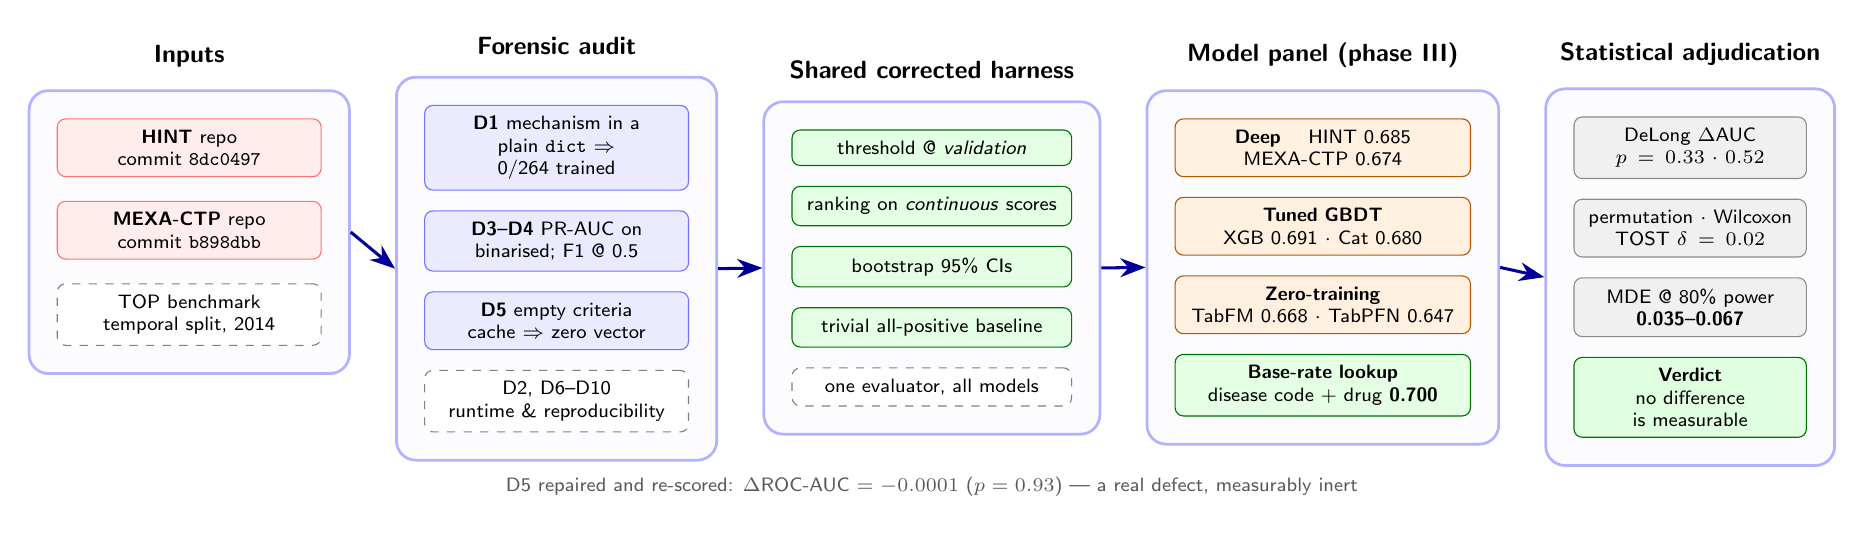
\begin{tikzpicture}[font=\sffamily,
  panel/.style={rounded corners=7pt, draw=blue!30, line width=1pt, fill=blue!1, inner sep=10pt},
  hdr/.style={font=\sffamily\bfseries\small, text=black},
  b/.style={rounded corners=3pt, draw=black!50, fill=black!4, align=center,
            inner xsep=5pt, inner ysep=4pt, font=\sffamily\scriptsize, text width=30mm},
  red/.style={b, draw=red!55, fill=red!7},
  blu/.style={b, draw=blue!55, fill=blue!8},
  grn/.style={b, draw=green!45!black, fill=green!10},
  yel/.style={b, draw=orange!70!black, fill=orange!12},
  gry/.style={b, draw=black!45, fill=black!6, text width=26mm},
  dsh/.style={b, dashed, fill=white},
  ar/.style={-{Stealth[length=3.2mm,width=2.4mm]}, line width=1.1pt, draw=blue!60!black}]
\node[red] (r1) {\textbf{HINT} repo\\\scriptsize commit \texttt{8dc0497}};
\node[red, below=3mm of r1] (r2) {\textbf{MEXA-CTP} repo\\\scriptsize commit \texttt{b898dbb}};
\node[dsh, below=3mm of r2] (r3) {TOP benchmark\\\scriptsize temporal split, 2014};
\begin{scope}[on background layer]
\node[panel, fit=(r1)(r2)(r3)] (P1) {};
\end{scope}
\node[hdr, above=1.5mm of P1] {Inputs};
\node[blu, right=13mm of r1.east, anchor=west] (d1) {\textbf{D1} mechanism in a\\plain \texttt{dict} $\Rightarrow$ 0/264 trained};
\node[blu, below=2.5mm of d1] (d3) {\textbf{D3--D4} PR-AUC on\\binarised; F1 @ 0.5};
\node[blu, below=2.5mm of d3] (d5) {\textbf{D5} empty criteria\\cache $\Rightarrow$ zero vector};
\node[dsh, below=2.5mm of d5, text width=30mm] (d10) {D2, D6--D10\\\scriptsize runtime \& reproducibility};
\begin{scope}[on background layer]
\node[panel, fit=(d1)(d3)(d5)(d10)] (P2) {};
\end{scope}
\node[hdr, above=1.5mm of P2] {Forensic audit};
\node[grn, right=13mm of d1.east, anchor=west, text width=32mm] (h1) {threshold @ \emph{validation}};
\node[grn, below=2.5mm of h1, text width=32mm] (h2) {ranking on \emph{continuous} scores};
\node[grn, below=2.5mm of h2, text width=32mm] (h3) {bootstrap 95\% CIs};
\node[grn, below=2.5mm of h3, text width=32mm] (h4) {trivial all-positive baseline};
\node[dsh, below=2.5mm of h4, text width=32mm] (h5) {one evaluator, all models};
\begin{scope}[on background layer]
\node[panel, fit=(h1)(h2)(h3)(h4)(h5)] (P3) {};
\end{scope}
\node[hdr, above=1.5mm of P3] {Shared corrected harness};
\node[yel, right=13mm of h1.east, anchor=west, text width=34mm] (m1) {\textbf{Deep} \quad HINT 0.685\\MEXA-CTP 0.674};
\node[yel, below=2.5mm of m1, text width=34mm] (m2) {\textbf{Tuned GBDT}\\XGB 0.691 $\cdot$ Cat 0.680};
\node[yel, below=2.5mm of m2, text width=34mm] (m3) {\textbf{Zero-training}\\TabFM 0.668 $\cdot$ TabPFN 0.647};
\node[grn, below=2.5mm of m3, text width=34mm] (m4) {\textbf{Base-rate lookup}\\disease code + drug \textbf{0.700}};
\begin{scope}[on background layer]
\node[panel, fit=(m1)(m2)(m3)(m4)] (P4) {};
\end{scope}
\node[hdr, above=1.5mm of P4] {Model panel (phase III)};
\node[gry, right=13mm of m1.east, anchor=west] (s1) {DeLong $\Delta$AUC\\\scriptsize $p=0.33$ $\cdot$ $0.52$};
\node[gry, below=2.5mm of s1] (s2) {permutation $\cdot$ Wilcoxon\\TOST $\delta=0.02$};
\node[gry, below=2.5mm of s2] (s3) {MDE @ 80\% power\\\textbf{0.035--0.067}};
\node[b, below=2.5mm of s3, draw=green!45!black, fill=green!12, text width=26mm]
     (s4) {\textbf{Verdict}\\no difference\\is measurable};
\begin{scope}[on background layer]
\node[panel, fit=(s1)(s2)(s3)(s4)] (P5) {};
\end{scope}
\node[hdr, above=1.5mm of P5] {Statistical adjudication};
\draw[ar] (P1.east) -- (P2.west);
\draw[ar] (P2.east) -- (P3.west);
\draw[ar] (P3.east) -- (P4.west);
\draw[ar] (P4.east) -- (P5.west);
\node[below=4mm of P3.south, font=\sffamily\scriptsize, text=black!65, align=center]
  {D5 repaired and re-scored: $\Delta$ROC-AUC $=-0.0001$ ($p=0.93$) --- a real defect, measurably inert};
\end{tikzpicture}}
\caption{Overview of the study. The two public implementations \citep{fu2022hint,zhang2025mexactp}
and the TOP benchmark enter a forensic audit that catalogues ten code-level defects; both models
are then re-evaluated under a single corrected harness, compared against a panel of deep, tuned
tabular, zero-training \citep{hollmann2025tabpfn,google2026tabfm} and historical base-rate
baselines, and adjudicated with tests of the \emph{difference} rather than overlapping intervals.
All values are phase-III test ROC-AUC.}
\label{fig:pipeline}
\end{figure*}

Figure~\ref{fig:pipeline} summarises the study end to end. Reading it left to right also states our
methodological position: we begin from the released artefacts rather than from reported numbers,
because the defects that matter here are visible only in code --- the same class of reproducibility
hazard that \citet{yang2026large} flag as the dominant vulnerability of benchmark-level (Level-2)
evidence, and that \citet{degrave2021ai} and \citet{geirhos2020shortcut} document in adjacent
clinical and vision settings. The harness stage exists because a defect in a \emph{reference}
model's evaluation propagates into every comparison drawn against it, and HINT is the reference for
this literature \citep{zhang2025mexactp,chen2024uq,wang2023spot}. The final stage is where our
verdict is decided: rather than reading winners off per-model confidence bands, we test the paired
difference and report a minimum detectable effect, the analogue of the pre-specification and
power discipline that clinical evaluation requires \citep{ylescupidez2023standardized,mentz2021clinical}.
\subsection{Related work}
\paragraph{The two models we re-evaluate.} HINT \citep{fu2022hint} relies on a hierarchical interaction network. It processes each trial through three parallel modalities. A message-passing network over SMILES graphs captures drug molecules. An ontology-aware ICD embedding handles target diseases. BioBERT reads the eligibility criteria. HINT then pushes these embeddings through pharmacology-knowledge modules---specifically, an ADMET block and a pharmacokinetic aggregator built from Highway networks. It fuses them in an interaction module before propagating the result through a dynamic attentive graph convolutional network, where the nodes represent the trial components. Its standard ablations---\texttt{Only\_Molecule}, \texttt{Only\_Disease}, \texttt{Interaction}, and \texttt{HINT\_nograph} (the full model with the graph removed)---let one isolate exactly what each modality contributes. We rely on these heavily in Section~\ref{sec:ablation}.
MEXA-CTP \citep{zhang2025mexactp} abandons this hand-built interaction graph entirely. Instead, it introduces a mode-experts design. Each modality projects and passes through its own self-attention ``expert.'' Learned routers then gate the resulting tokens, penalized by a Cauchy sparsity loss. Cross-attention blocks exchange information between every ordered pair of modes. A contrastive loss aligns these paired cross-attended representations. Finally, a compensation self-attention block pools them, and a linear head predicts the outcome. Contrary to what one might assume, the two models do \emph{not} share encoders (Table~\ref{tab:encoders}): HINT encodes molecules with a D-MPNN and diseases with the GRAM ICD ontology, whereas MEXA-CTP as published uses a DeepChem molecular featuriser and the \texttt{icdcodex} disease embedding, and our own retraining standardises the front-end differently again (MACAW molecule vectors, \texttt{icd2vec}); only the BioBERT criteria encoder is common to all three, and even that differs in granularity (paragraph- vs statement-level). What the two models genuinely share is the TOP benchmark and task; their headline architectural difference is how they model cross-modal interaction --- a hand-built graph in HINT versus routed cross-attention in MEXA-CTP --- which our audit isolates. Because the encoders are not held identical, the comparison also carries an encoder confound; we note it here and in the limitations, but since no between-model difference is detectable in the first place (Section~\ref{sec:power}), differing encoders cannot manufacture a gap that does not exist.
\paragraph{Mixture-of-experts and the missing isolation test.} Mixture-of-experts (MoE) architectures have gained prominence here on the promise of modeling distinct trial modalities (molecule, disease, protocol) through specialized subnetworks. However, if a paper claims its experts genuinely learn discriminative, contributing representations, it must explicitly isolate their contribution. In an adjacent domain, a glioblastoma MoE survival model (three experts and a gating network) did exactly this. The authors collapsed their MoE design into a single-expert network and reported the discrimination drop from AUC $0.839$ to $0.806$ ($-3.9\%$) \citep{reyes2026therapeutic}. That is a measurable architectural contribution. Models advancing MoE claims for clinical trial outcome prediction provide no such isolation test. Our forensic audit reveals exactly why: the code made it impossible. The developers stored the cross-attention, self-attention, and router layers in a plain Python \texttt{dict} rather than an \texttt{nn.ModuleDict}. Consequently, PyTorch never registered these submodules. They never entered the optimizer. They were never written to the \texttt{state\_dict} checkpoints (Section~\ref{sec:defects}). The mechanism never trained, including in the original authors' own runs. Here, we fix the implementation and report the first actual evaluation of this mechanism.
\paragraph{Benchmark lineage.} The TOP benchmark was curated alongside HINT \citep{fu2022hint}. Its binary outcome labels are not algorithmic: the HINT paper states verbatim that ``[t]rial outcome labels (binary labels) are extracted through manual curation by an internal IQVIA team,'' with the raw trial variables parsed from ClinicalTrials.gov XML and the sets time-split at January~1, 2014 \citep{fu2022hint}. We flag this because it is easy to misattribute: COMPOSE \citep{gao2020compose}, a cross-modal pseudo-siamese patient--trial matching network, is a \emph{baseline} HINT compares against, not the source of the labels --- a distinction we verified against the source paper. It is worth stating plainly what the label means, because it bounds how high any ROC-AUC can go. ``Success'' in TOP is not trial completion and not a single clean regulatory event: it is a hand-curated IQVIA determination of whether the trial met its endpoint / the drug progressed, aggregated across heterogeneous trial types. Such a label is inherently noisy --- human-curated, and part of the modest $0.685$ ceiling we and everyone else observe is almost certainly label noise rather than model weakness --- a reason to be sceptical of \emph{small} reported gains, and an argument that the benchmark's own labels, not just its models, deserve audit. Since its release, HINT has become both the reference baseline \citep{zhang2025mexactp} and the base on which new methods are built. For example, UQ-HINT \citep{chen2024uq} adds selective classification on top of HINT's outputs, and therefore inherits its exact evaluation code.
\paragraph{HINT's successor literature.} The line of work built on TOP extends well beyond
MEXA-CTP, and our audit of the benchmark's labels, split and metrics bears on all of it. SPOT
\citep{wang2023spot} clusters trials into topics and adds a meta-learning module over the same
labels; Trial2Vec \citep{wang2022trial2vec} learns self-supervised trial-document embeddings
used downstream for outcome tasks; and TrialBench \citep{chen2025trialbench} --- from the HINT
authors --- packages $23$ ClinicalTrials.gov-derived datasets across eight tasks, including
trial-approval prediction, in the same tabular/multi-modal form we examine here. Each inherits
the label provenance and small per-phase test sizes that Sections~\ref{sec:dataquality}
and~\ref{sec:power} show cap what is measurable; a shared, power-aware evaluation protocol is
therefore relevant to the successor benchmarks, not only to HINT and MEXA-CTP.
\paragraph{Is the molecular modality necessary?} LINT \citep{gao2024lint} predicts trial approval strictly from text. It encodes the trial description and eligibility text using a BioBERT-style language model over a GRAM disease-ontology representation, discarding the molecular graph entirely. In Section~\ref{sec:ablation}, we show that HINT's drug branch alone performs near chance, while its disease branch alone matches the full model. This provides independent, ablation-based confirmation of what LINT demonstrates from the architecture side: the structural molecular signal adds negligible value.
\paragraph{Tabular foundation models as a baseline.} A recent line of work trains a single transformer to perform supervised learning on arbitrary tables by in-context learning: it predicts a test row after being shown the training rows as context, with no gradient training at inference \citep{hollmann2025tabpfn,google2026tabfm}. Because trial metadata, disease-ontology codes, and molecular physicochemical descriptors are all naturally tabular, such a model is a strong, assumption-light baseline for the TOP task---it consumes the same information HINT does, minus the graph structure, at zero training cost. We use it in Section~\ref{sec:tabfm} as the most modern member of a broad tabular-baseline panel.
\paragraph{Accuracy versus benefit.} Even a correctly measured gain might not help real patients. The ORACLE trial \citep{fritz2024effect} showed clinicians a model's predictions. The clinicians agreed with the model more often, but their actual \emph{accuracy} did not improve. The authors blamed data drift, concept drift, and automation bias. Similarly, \citet{jayakumar2025shared} deployed a model trained on 700{,}000 patients into a randomized trial simply to test if decision quality improved in practice. Our claim operates one step prior in that chain: before we ask if a gain helps anyone, we must first prove the gain is measurable.
\paragraph{Metric discipline in clinical statistics.} Clinical trials require researchers to pre-specify their outcome metrics and adjust for known baseline covariates \citep{ylescupidez2023standardized}. When evaluated strictly, classical statistical models remain highly competitive \citep{mentz2021clinical}. Our findings in Section~\ref{sec:baselines} mirror this reality perfectly. In machine learning, locking down every free choice (like decision thresholds) on a validation set is the exact analogue of clinical pre-specification. We enforce that discipline here.
% =====================================================================
\section{Methods}
\label{sec:methods}
\subsection{What makes the published comparison ill-posed}
The published comparison measures the two models under completely different rules. Worse, several of those rules are simply wrong. Five specific problems compound to invalidate the results:
\begin{enumerate}[leftmargin=1.4em,itemsep=1pt,topsep=2pt]
\item \textbf{Different model-selection criteria (a code-versus-paper discrepancy).} The MEXA-CTP paper states that the best training epoch is chosen on validation, but the released code selects it on the \emph{test} ROC-AUC. HINT selects its epoch on \emph{validation}, consistent with its description. We flag the MEXA-CTP case specifically as a mismatch between the published protocol and the shipped implementation --- not as a stated design choice --- because it is the implementation that produced the reported numbers. Choosing a checkpoint on the same set used for final scoring leaks the test labels into training and inflates the reported performance; the two models are then not even selected by the same procedural logic, let alone the same data splits.
\item \textbf{Fixed $0.5$ threshold.} Both models report their F1 scores using a hard-coded $0.5$ decision cutoff. However, the benchmark's positive rate fluctuates wildly---from $0.55$ in phase~I up to $0.75$ in phase~III. Under these conditions, a fixed threshold forces F1 to measure the underlying class prior rather than the actual ranking quality. To prove this, we simply recalibrated the threshold on validation data. That one change alone boosted HINT's phase~I F1 score by $+0.119$ (Section~\ref{sec:results}).
\item \textbf{PR-AUC on binarised predictions.} HINT computes its PR-AUC only after thresholding the raw predictions into strict $0/1$ labels, instead of using the continuous scores. This calculation error understates the true PR-AUC by anywhere from $0.020$ to $0.081$. Far more dangerously, it completely \emph{reorders} the performance rankings of the models (Section~\ref{sec:metricweak}).
\item \textbf{No trivial baseline.} Neither paper reports an all-positive reference score. Without this trivial baseline, the absolute F1 numbers become meaningless. For instance, achieving an F1 of $0.86$ sounds impressive on paper. Yet, on a test set with $0.75$ positive labels, simply guessing ``every trial succeeds'' yields the exact same score.
\item \textbf{The wrong kind of uncertainty, and no test of the difference.} MEXA-CTP does report a $\pm$ in its tables, but it is a \emph{test-resampling} bootstrap sd over $10$ samples of a \emph{single} model --- not the two quantities that decide whether a gain is real: the \emph{training-seed} variance (re-running the same model from a different seed) and a paired \emph{test of the difference} between two models. Reporting a per-model bootstrap band and then reading off a winner from non-overlapping bands is exactly the error Section~\ref{sec:power} corrects: two bands can overlap while the paired difference is significant, and vice versa. On a benchmark where the sampling noise on a between-model \emph{difference} (DeLong SE $\approx0.018$) is comparable to or larger than the $\sim0.01$--$0.03$ effect sizes claimed, the missing difference test is the omission that matters most.
\end{enumerate}
Each of these defects works independently to either flatter the more complex model or mask the random noise that would otherwise undercut its claims. Combined, they ensure the published comparison is not just imprecise, but fundamentally ill-posed.
\subsection{Shared evaluation harness}
We run each model entirely in its own environment. The two repositories never share code and never import one another. Instead, each model simply writes its raw, per-trial predictions (\texttt{nctid}, score, label, split) to disk for both the validation and test sets. A single, independent evaluator then reads these files and applies the exact same rules to every model:
\begin{itemize}[leftmargin=1.4em,itemsep=1pt,topsep=2pt]
\item \textbf{Threshold selection.} We calibrate each model purely on its \emph{own validation} predictions. The harness scans the midpoints between adjacent validation scores to find the exact threshold that maximizes F1. We then freeze that threshold and apply it to the test set. This means HINT can safely emit sigmoid probabilities while MEXA-CTP outputs raw logits. The absolute score offset does not matter; the harness evaluates each model fairly on its own scale.
\item \textbf{Ranking metrics.} We compute ROC-AUC and PR-AUC strictly on \emph{continuous} scores. We never binarize the predictions before ranking them. This makes the metrics invariant to the underlying score scale and completely bypasses the PR-AUC defect identified earlier.
\item \textbf{Uncertainty.} We generate $95\%$ confidence intervals using $1000$ bootstrap resamples of the test set. We fix the random seed to guarantee these intervals remain perfectly reproducible.
\item \textbf{Reference.} Every results table includes a trivial, all-positive baseline. This forces the reader to interpret any reported F1 score against the performance of a dummy model that simply ignores the input and guesses positive for every trial under the exact same class imbalance.
\end{itemize}
Under this architecture, neither repository evaluates itself. The final numbers flow entirely from the shared harness reading raw prediction files. This setup makes it structurally impossible for two repositories to make the same mistake in different ways. The evaluation logic might still contain a flaw, but it can now only hide in \emph{one} place. And that single place is fully auditable. The same harness scores the tabular baselines of Section~\ref{sec:tabfm}, which are simply additional prediction files, so every model in this paper---deep or tabular---is judged by one protocol.
\subsection{Data and protocol}
We force both models to operate on the exact same TOP benchmark splits (Table~\ref{tab:splits}). We freeze the global random seed at 2023. For the input data representations, we rely on the 2024 version of the ICD-10-CM hierarchy and embed the disease codes into 64 dimensions using \texttt{icd2vec}. We map drug molecules into 15-dimensional SMILES embeddings via MACAW, specifically locking \texttt{random\_state=2023} to guarantee deterministic outputs. We encode all eligibility criteria text using BioBERT (\texttt{dmis-lab/biobert-v1.1}).
These are our harness's inputs; they are not identical to either model's published encoders,
which is why the per-modality encoders differ across the three configurations
(Table~\ref{tab:encoders}). We standardise the split, protocol and metrics --- not the
front-end encoders --- so the encoder difference remains a confound we flag rather than remove.
\begin{table}[t]
\centering\small
\caption{The models do \emph{not} share encoders. Only the BioBERT criteria encoder is common,
and at different granularities. This is an encoder confound, flagged in the text; it cannot
create a between-model difference because none is detectable (Section~\ref{sec:power}).}
\label{tab:encoders}
\begin{tabular}{llll}
\toprule
Modality & HINT (published \& our run) & MEXA-CTP (published) & MEXA-CTP (our retrain) \\
\midrule
Molecule & D-MPNN over SMILES graph & DeepChem featuriser & MACAW ($15$-d) \\
Disease  & GRAM (ICD ontology) & \texttt{icdcodex} & \texttt{icd2vec} ($64$-d) \\
Criteria & BioBERT (paragraph) & BioBERT (statement) & BioBERT (\texttt{biobert-v1.1}) \\
\bottomrule
\end{tabular}
\begin{minipage}{\linewidth}\vspace{2pt}\scriptsize Sources: HINT \citep{fu2022hint} and
MEXA-CTP \citep{zhang2025mexactp} papers/repositories; our-retrain column from this harness
(Section~\ref{sec:methods}). \end{minipage}
\end{table}
During training, we sweep the learning rate identically for both architectural arms. We select the optimal epoch based entirely on validation performance, enforcing early stopping with a patience of 10.
\begin{table}[t]
\centering
\small
\caption{Evaluation splits and class balance. Note the severe shift in positive rate between validation and test (especially in Phase III), which naturally limits how well any validation-selected threshold can transfer to the final evaluation.}
\label{tab:splits}
\begin{tabular}{lccccc}
\toprule
 & Train & Valid $n$ & pos.\ rate & Test $n$ & pos.\ rate \\
\midrule
Phase~I & 1044 & 117 & 0.573 & 627 & 0.553 \\
Phase~II & 4005  & 446 & 0.466 & 1654 & 0.555 \\
Phase~III & 3094 & 344 & 0.666 & 1146 & 0.750 \\
\bottomrule
\end{tabular}
\end{table}
\paragraph{A prior discrepancy: MEXA-CTP's reported dataset matches neither the shipped data nor
its own results.} Before any code-level defect, MEXA-CTP's stated dataset is internally
inconsistent. Its Table~1 reports per-phase (training / test / success-ratio) of
$1{,}088/312/70\%$ (I), $2{,}611/789/33\%$ (II) and $4{,}313/1{,}147/30\%$ (III), under
per-phase 2014 split days. But the data actually shipped in MEXA-CTP's own repository
(\texttt{DataPath/\{trainphase,validphase,test\}/phase\_*}) contains \emph{exactly} the HINT TOP
counts of Table~\ref{tab:splits} --- $1044/117/627$ (I), $4005/446/1654$ (II), $3094/344/1146$
(III), with test positive rates $0.553/0.555/0.750$. The two disagree in every phase: the
reported phase~I and~II test sets ($312$, $789$) are roughly \emph{half} the shipped ones
($627$, $1654$), and the reported success ratios ($70/33/30\%$, \emph{decreasing} with phase)
are not the shipped positive rates ($55/55/75\%$, \emph{increasing} with phase). Which split
underlies the reported numbers is then settled by the results themselves: MEXA-CTP's Table~2
lists HINT at ROC-AUC $0.573/0.621/0.685$ for phases~I/II/III --- matching our HINT run on the
shipped split ($0.574/0.621/0.685$) to within $0.001$, not any split of the Table~1 sizes. The
reported metrics were therefore computed on the shipped HINT split, while Table~1 describes a
\emph{different}, unused split. This is a more basic reproducibility problem than any single
code bug: the paper's documented dataset does not describe the data underlying its own results.
We evaluate every model in this paper on the shipped counts of Table~\ref{tab:splits}, which are
also the counts behind MEXA-CTP's reported HINT baseline.
% =====================================================================
\section{Defects}
\label{sec:defects}
\begin{table*}[t]
\centering\small
\caption{Master list of the ten code-level defects found (D1--D5 substantive, D6--D10
secondary/runtime), with the consequence of each. Every defect mentioned in the text
references its ID here.}
\label{tab:defects}
\begin{tabular}{clp{4.3cm}l}
\toprule
ID & Defect & Consequence & Evidence \\
\midrule
D1 & Attention/routers in plain \texttt{dict} (MEXA) & Invisible to the optimizer ($0/264$ tensors), unchanged after a backward+step, and absent from every checkpoint & Table~\ref{tab:paramreg} \\
D2 & Full-masking $\rightarrow$ NaN (MEXA) & NaN at every lr that trains; with a minimal guard, training survives but every sequence collapses to a single token & Table~\ref{tab:collapse}\\
D3 & PR-AUC on binarised predictions (HINT) & Understates by $0.020$--$0.081$; reorders variants & Table~\ref{tab:praucbug} \\
D4 & Threshold hard-coded at $0.5$ & F1 reports the class prior & Table~\ref{tab:f1} \\
D5 & Empty \texttt{sentence2embedding.pkl} (HINT) & HINT's eligibility-criteria branch returns a zero $768$-vector for every trial; the modality is silently dead & \S\ref{sec:defects} (6-byte empty dict) \\
D6 & \texttt{.to(get\_device())} hard-codes GPU (MEXA) & Model cannot run on CPU & Runtime error \\
D7 & Ablation variants miss \texttt{device} in \texttt{super()} (HINT) & Two variants un-instantiable & Type error \\
D8 & Published lr $5\times10^{-2}$ diverges once attention trains (MEXA) & Survived only because those params were frozen (D1) & \texttt{runs\_summary.csv} \\
D9 & \texttt{squeeze()} collapses the batch dim when $B{=}1$ (MEXA) & Silent shape bug & Runtime \\
D10 & Checkpoint load fails under PyTorch $\ge2.6$ & Reproducibility break & Runtime \\
\bottomrule
\end{tabular}
\end{table*}
\begin{table}[t]
\centering\small
\caption{Parameter registration for the interaction mechanism. In the original
plain-\texttt{dict} model the self-attention, cross-attention and router sub-modules are
invisible to \texttt{named\_parameters()}, so none of the $264$ mechanism tensors reach the
optimizer and none change after a backward+step. The \texttt{nn.ModuleDict} fix registers
all of them; all $144$ cross-attention tensors are then updated. The released checkpoints
serialise only $48$--$49$ keys, none of them attention or router. A single backward+step
suffices as proof: a tensor absent from the optimizer cannot change at any step, so the
zero update generalises to all of training without a full run.}
\label{tab:paramreg}
\begin{tabular}{lccccc}
\toprule
Configuration & self-att & cross-att & routers & trainable params & cross-att in opt. / changed \\
\midrule
Original (plain \texttt{dict})   & 0  & 0   & 0  & 312{,}034 & 0/144 \\
Fixed (\texttt{nn.ModuleDict})   & 72 & 144 & 48 & 319{,}562 & 144/144 \\
\midrule
\multicolumn{6}{l}{Released checkpoints: phase I $49$, phase II $48$, phase III $49$ keys --- $0$ mechanism keys in each.} \\
\bottomrule
\end{tabular}
\end{table}
We do not need to train the buggy model to prove it never learns: ``never trained'' and
``never saved'' are not stochastic outcomes but a deterministic consequence of PyTorch's
module semantics. A plain \texttt{dict} is not registered as a submodule, so its parameters
never enter \texttt{named\_parameters()} --- the exact iterator that both the optimizer and
\texttt{state\_dict()} consume. The tensors therefore cannot receive gradients, cannot be
updated, and cannot be serialised, regardless of the data, learning rate, or number of
epochs. Table~\ref{tab:paramreg} is confirmation of this at three levels ($0$ tensors in the
optimizer, $0$ changed after a backward+step, $0$ mechanism keys in every released
checkpoint), not a run that merely happened to fail. The released checkpoints also serialise
the optimizer state alongside the weights, and it tracks exactly the $48$ trainable
non-mechanism tensors with no moment buffers for any attention or router parameter: the
Adam optimizer never even allocated state for the mechanism, because it never entered the
optimizer in the first place.
\paragraph{An entire modality silently zeroed (D5).} The shipped
\texttt{data/sentence2embedding.pkl} --- HINT's cache of BioBERT sentence embeddings for the
eligibility criteria --- is an empty dictionary (6 bytes). \texttt{protocol2feature} looks up
each criterion sentence in this dictionary and, finding nothing, falls back to
\texttt{torch.zeros(1,768)}: HINT's eligibility-criteria modality returns an all-zero vector
for \emph{every} trial. Any run from the public repository (ours included) therefore trains
and evaluates HINT with a dead criteria branch unless the cache is regenerated.
\emph{We repaired the cache and measured the effect.} Regenerating the full BioBERT criteria
cache ($513{,}863$ sentence embeddings, \texttt{dmis-lab/biobert-v1.1}) and re-scoring the
released HINT checkpoint with a \emph{live} criteria branch changes its phase-III performance by
nothing: ROC-AUC $0.6850$ vs $0.6851$ (paired $\Delta=-0.0001$, $95\%$ CI $[-0.0017,+0.0016]$,
$p=0.93$) and PR-AUC $0.8519$ vs $0.8517$ ($\Delta=+0.0002$, $p=0.78$); the HINT$-$MEXA gap is
identical to four decimals ($+0.1671$ either way). The empty cache is thus a genuine defect --- a
whole modality is silently dead --- but a \emph{quantifiably inert} one: feeding real
eligibility-criteria embeddings in place of zeros moves HINT's numbers by $0.0001$. We verified
that this is a real substitution, not a silent no-op: with the regenerated cache the criteria
branch emits a non-zero embedding (mean L2 norm $>0$) for every trial, versus an exact zero vector
before. This strengthens rather than complicates the paper's thesis: HINT's released output is
\emph{empirically} unchanged by activating its criteria modality (we say ``empirically'', not
``provably'' --- this is a measurement on the released checkpoint, not a proof), so its signal is
carried in practice by the disease codes (Section~\ref{sec:ablation}), and none of the published
MEXA-CTP-over-HINT advantage can be attributed to D5 degrading HINT's evaluation. (This is the released-checkpoint re-scoring; a
full retrain-from-scratch with the live cache is the one remaining check, currently blocked by
defect~D10 --- \texttt{torch.load} failing under PyTorch~$\ge2.6$ --- a fitting obstacle. We do
not expect it to change the verdict, since even feeding the live branch to the trained model
changes nothing.) Two careful corollaries survive: we still do not claim eligibility-criteria
\emph{text} is uninformative in general --- only that HINT does not use it --- and our tabular
protocol's criteria \emph{counts} (Section~\ref{sec:tabfm}), computed directly from the text,
are unaffected by D5 and already carry a shallow criteria signal.

\paragraph{Secondary defects (D6--D10).} The published learning rate $5\times10^{-2}$ diverges
once the attention actually trains (D8; it survived only because those parameters were frozen
by D1); a \texttt{squeeze()} collapses the batch dimension when $B=1$ (D9); checkpoint loading
fails under PyTorch $\geq$ 2.6 (D10); and two device-placement bugs (D6, D7) block CPU
execution and the instantiation of two ablation variants.
\subsection{Two defects concealing each other}
\label{sec:twobugs}
The Cauchy loss exists to push routing probabilities toward zero, and the masking step
removes tokens whose probability falls below $\tau$. If all tokens of a sequence fall below
$\tau$, the attention mask becomes fully saturated, softmax is taken over an all-$-\infty$
row, and the output is NaN. This was never observed because D1 froze the router
\emph{weights} at their initialisation. We are precise about what ``frozen'' does and does not
imply: the Cauchy sparsity loss is still computed each step and its gradient still flows
\emph{through} the router into the encoder parameters, which do train --- so the loss is not
literally inert, and MEXA-CTP's own reported effect of the routing loss on the learned
representation is consistent with that encoder-side gradient. What never happens is the part
the mechanism depends on: the router itself never adapts. Held at a fixed random projection,
it cannot learn to drive tokens below $\tau$, so routing probabilities stay near their
initialisation and the masking saturation that produces the NaN never occurs in the authors'
runs. The correction is therefore not ``the sparsification loss did nothing'' but ``the
sparsification loss could shape the encoders yet never trained the router, so the adaptive
routing the paper describes never operated and its failure mode never surfaced.''
\textbf{D1 is thus the reason training did not crash.} Repairing either defect alone
produces a model that either does nothing or fails; both must be addressed together, which
is why no prior work---including the original authors'---ever tested the mechanism the
paper is about.
Instrumenting the masking step (phase~II, seed~2023) confirms this is deterministic rather
than a numerical accident: without a guard the first NaN appears at step $9$, $28$ and $184$
for learning rates $5\times10^{-2}$, $10^{-2}$ and $10^{-3}$, and the fraction of tokens
driven below $\tau$ by step~$300$ rises from $13\%$ at $10^{-4}$ to $100\%$ at
$5\times10^{-2}$. A minimal guard that always keeps the highest-probability token removes
the NaN but not the collapse: at $5\times10^{-2}$ the mean routing probability falls to
$0.003$ and every sequence is reduced to a single surviving token, so the cross-attention
the paper studies operates over one token. The architecture can be kept numerically alive,
but not architecturally.
\begin{table}[t]
\centering\small
\caption{Masking collapse on phase~II (seed 2023, 300 steps). Without the guard, the
first NaN appears earlier as the learning rate grows; the guard removes the NaN but the
routing probabilities still collapse, leaving essentially one token per sequence.
$^\dagger$Measured at the NaN step for diverged runs, or at step 300 for $10^{-4}$.}
\label{tab:collapse}
\begin{tabular}{lccccc}
\toprule
& \multicolumn{2}{c}{no guard} & \multicolumn{3}{c}{with guard @ step 300} \\
\cmidrule(lr){2-3}\cmidrule(lr){4-6}
lr & first NaN step & below-$\tau$ frac$^\dagger$ & mean router $p$ & below-$\tau$ frac & final loss \\
\midrule
$5\times10^{-2}$ & 9   & 1.00 & 0.003 & 1.00 & 0.721 \\
$1\times10^{-2}$ & 28  & 0.88 & 0.011 & 1.00 & 0.610 \\
$1\times10^{-3}$ & 184 & 0.81 & 0.088 & 0.97 & 0.652 \\
$1\times10^{-4}$ & none & 0.13 & 0.379 & 0.13 & 0.921 \\
\bottomrule
\end{tabular}
\end{table}
% =====================================================================
\section{Results}
\label{sec:results}
\subsection{A fair, corrected comparison}
With the shared harness and the defect fixes of Section~\ref{sec:methods} in place, the HINT
versus MEXA-CTP comparison is finally well-posed. We put three questions to it in turn: how the
two models compare head-to-head on phase~III under one protocol; whether MEXA-CTP's central
cross-attention mechanism contributes anything once it is actually trained; and where HINT's own
predictive signal comes from once its modalities are ablated. As the next three parts show, the
answers are, respectively, no measurable difference, nothing, and the disease codes alone.
\subsubsection{The head-to-head result}
\begin{table*}[t]
\centering
\small
\caption{Phase~III test performance under the shared corrected protocol. Thresholds are selected on validation; ranking metrics use continuous scores. \textbf{The two uncertainty types are not comparable and are kept in separate columns:} for HINT, brackets are \emph{test-resampling} bootstrap $95\%$ CIs (single run); for the retrained MEXA-CTP arms, $\pm$ is \emph{training-seed} sd over 7 seeds at the matched configuration ($\rho_1{=}0.05$, $\rho_2{=}0.01$, $\tau{=}0.3$). The released checkpoint and trivial rows are single points. See Section~\ref{sec:power} for why these sources must not be read against each other.}
\label{tab:fair}
\begin{tabular}{lccc}
\toprule
Model & ROC-AUC & PR-AUC & F1 \\
\midrule
HINT (run~A), \emph{test-resample CI} & 0.685 {\scriptsize [0.647, 0.720]} & 0.852 {\scriptsize [0.824, 0.878]} & 0.826 {\scriptsize [0.806, 0.845]} \\
MEXA (retrained \emph{buggy}), \emph{seed sd} & 0.674 $\pm$ 0.015 & 0.853 & 0.838 \\
MEXA (retrained \emph{fixed}), \emph{seed sd} & 0.674 $\pm$ 0.011 & 0.850 & 0.846 \\
MEXA (released checkpoint), \emph{point} & 0.518 & 0.788 & 0.809 \\
\textsc{Trivial} (all-positive), \emph{point} & 0.500 & 0.750 & \textbf{0.857} \\
\bottomrule
\end{tabular}
\begin{minipage}{\linewidth}\vspace{2pt}\scriptsize Source: \texttt{results\_phase\_III.csv}; MEXA arms from \texttt{ab\_test\_results\_phase\_III.csv} (deduplicated on arm/seed/config); released checkpoint from \texttt{seed\_sensitivity\_phase\_III.csv}. No model exceeds the trivial baseline on F1. \end{minipage}
\end{table*}
Table~\ref{tab:fair} gives phase~III. The released MEXA-CTP checkpoint is statistically
indistinguishable from random ranking. Because its attention weights were never saved,
every load draws fresh random values, and this reload variance holds across all three
phases (Table~\ref{tab:reload}): ROC-AUC spans a range of $0.055$--$0.117$ over five seeds,
larger than the reported gains, and one seed in five falls below $0.5$ in every phase. With
the checkpoint's hard-coded $0.5$ threshold the F1 is more volatile still, its range reaching
$0.65$ (phase~I) and $0.48$ (phase~III) across reloads of a \emph{single} checkpoint --- a
metric this unstable cannot support the reported $11.3\%$ improvement.
\begin{figure}[htbp]
\centering
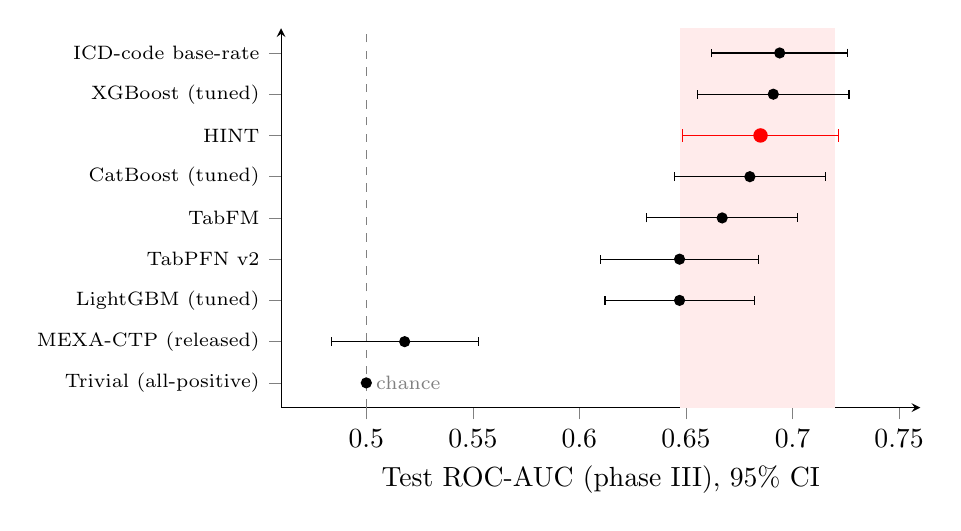
\begin{tikzpicture}
\begin{axis}[
  width=0.8\linewidth, height=6.4cm,
  xmin=0.46, xmax=0.76,
  xlabel={Test ROC-AUC (phase~III), 95\% CI},
  ytick={0,1,2,3,4,5,6,7,8},
  yticklabels={{Trivial (all-positive)},{MEXA-CTP (released)},{LightGBM (tuned)},{TabPFN~v2},{TabFM},{CatBoost (tuned)},{HINT},{XGBoost (tuned)},{ICD-code base-rate}},
  y tick label style={font=\scriptsize}, ymin=-0.6, ymax=8.6,
  axis lines=left, tick align=outside, enlarge y limits=false,
  every axis plot/.append style={thick},
]
\fill[red!8] (axis cs:0.647,-0.6) rectangle (axis cs:0.720,8.6);
\draw[gray,dashed] (axis cs:0.5,-0.6) -- (axis cs:0.5,8.6);
\node[gray,anchor=south west,font=\scriptsize] at (axis cs:0.5,-0.4){chance};
\addplot[only marks,mark=*,black,mark size=1.6pt,
  error bars/.cd,x dir=both,x explicit]
  coordinates {(0.500,0) (0.518,1)+-(0.0345,0) (0.647,2)+-(0.035,0)
  (0.647,3)+-(0.037,0) (0.667,4)+-(0.0355,0) (0.680,5)+-(0.0355,0)
  (0.691,7)+-(0.0355,0) (0.694,8)+-(0.032,0)};
\addplot[only marks,mark=*,red,mark size=2.2pt,
  error bars/.cd,x dir=both,x explicit] coordinates {(0.685,6)+-(0.0365,0)};
\end{axis}
\end{tikzpicture}
\caption{Phase-III test ROC-AUC with $95\%$ CIs for every model considered: the two deep
models (HINT, MEXA-CTP), two zero-training foundation models (TabFM, TabPFN~v2), three tuned
gradient-boosting baselines, and a ten-line disease-code base-rate lookup. The CIs are shown for
orientation only; inference is by the paired DeLong test (Section~\ref{sec:power}), under which
no model differs significantly from HINT (HINT$-$TabFM $p=0.33$, HINT$-$GradBoost $p=0.052$,
HINT$-$base-rate $p=0.52$). Only the released MEXA-CTP checkpoint (near chance) is clearly
worse; the base-rate lookup and tuned XGBoost sit, if anything, marginally above HINT.}
\label{fig:forest}
\end{figure}
\begin{table}[t]
\centering\small
\caption{Reload variance of the released MEXA-CTP checkpoint: the same file evaluated under
five seeds. Since the attention/router weights were never saved, each load re-randomises
them. ROC-AUC ranges exceed the improvements the original reports, and F1 (at the
checkpoint's fixed $0.5$ threshold) swings across most of its range.}
\label{tab:reload}
\begin{tabular}{lcccc}
\toprule
Phase & ROC-AUC range & sd & F1@0.5 range & seeds ROC $>0.5$ \\
\midrule
I   & $0.490$--$0.578$
($0.087$)& $0.034$ & $0.050$--$0.698$
($0.648$)& 4/5 \\
II  & $0.454$--$0.571$
($0.117$)& $0.046$ & $0.370$--$0.717$
($0.346$)& 4/5 \\
III & $0.478$--$0.534$
($0.055$)& $0.023$ & $0.380$--$0.857$
($0.477$)& 4/5 \\
\bottomrule
\end{tabular}
\begin{minipage}{\linewidth}\vspace{2pt}\scriptsize Source: ROC-AUC and sd from \texttt{seed\_sensitivity\_phase\_\{I,II,III\}.csv} (5 reload seeds each); F1 ranges recomputed at the fixed $0.5$ threshold from \texttt{preds/\_seedtest\_mexa\_phase\_\{I,II,III\}\_seed*.csv}. \end{minipage}
\end{table}
\subsubsection{Does training the cross-attention help?}
\begin{table*}[t]
\centering
\small
\caption{Effect of actually training the cross-attention. Runs are matched on $(\rho_1,\rho_2,\tau,\text{seed})$ and de-duplicated before pairing. The sign is the opposite of a useful mechanism (buggy $\ge$ fixed); the only powered cell (phase~III) is not significant.}
\label{tab:ab}
\begin{tabular}{lccc}
\toprule
Subset & \#pairs & $\Delta$ (buggy $-$ fixed) & $p$ \\
\midrule
Phase~I & 2 & +0.0320 & --- \\
Phase~II & 3 & +0.0101 & --- \\
Phase~III & 7 & +0.0004 & 0.964 \\
\bottomrule
\end{tabular}
\begin{minipage}{\linewidth}\vspace{2pt}\scriptsize Source: \texttt{ab\_test\_results\_phase\_\{I,II,III\}.csv}, deduplicated on (arm, seed, config) then paired on seed. $p$ is a paired $t$-test on phase~III only; phases~I--II ($n{=}2,3$) are descriptive, and we do \emph{not} pool across phases (different prevalences, sizes and effects --- not exchangeable). \end{minipage}
\end{table*}
It does not (Table~\ref{tab:ab}). MEXA-CTP has three loss/routing hyperparameters: the Cauchy
routing-sparsity weight $\rho_1$, the NT-Xent contrastive weight $\rho_2$, and the routing
threshold $\tau$. Pairing runs matched on $(\rho_1,\rho_2,\tau,\text{seed})$,
the buggy arm---in which the cross-attention is frozen at its random initialisation---is if
anything \emph{higher} than the fixed arm that actually trains it: $\Delta=+0.032$ (phase~I),
$+0.010$ (phase~II) and $+0.0004$ (phase~III, $p=0.96$, the only cell with enough pairs to
test). The effect is never negative and never significant, the opposite of what a useful
mechanism would produce; we neither test the $n{=}2,3$ phases nor pool across the three, which
are not exchangeable. The two other components that distinguish MEXA-CTP from a
plain encoder are equally inert: sweeping the routing threshold $\tau$ from $0.0$ to $0.5$
moves phase~III ROC-AUC only from $0.685$ to $0.669$, and the contrastive weight $\rho_2$
from $0$ to $0.1$ moves it from $0.678$ to $0.688$---both well inside a single seed's
confidence interval ($\pm0.035$). Every architectural component that distinguishes MEXA-CTP
from a plain encoder can be disabled, frozen, or retuned without measurable cost.
\subsubsection{HINT's ablation ladder is flat}
\label{sec:ablation}
\begin{table*}[t]
\centering
\small
\caption{HINT ablation ladder (test ROC-AUC, 95\% CI). The disease branch alone matches the full model in every phase; the drug branch alone is near chance.}
\label{tab:ablation}
\begin{tabular}{lccc}
\toprule
Variant & Phase~I & Phase~II & Phase~III \\
\midrule
Only\_Molecule & 0.583 {\scriptsize [0.539, 0.626]} & 0.548 {\scriptsize [0.521, 0.576]} & 0.540 {\scriptsize [0.501, 0.579]} \\
Only\_Disease & 0.573 {\scriptsize [0.531, 0.616]} & 0.626 {\scriptsize [0.599, 0.652]} & 0.700 {\scriptsize [0.663, 0.735]} \\
Interaction & 0.557 {\scriptsize [0.512, 0.602]} & 0.619 {\scriptsize [0.592, 0.647]} & 0.711 {\scriptsize [0.674, 0.743]} \\
HINT\_nograph & 0.586 {\scriptsize [0.541, 0.631]} & 0.619 {\scriptsize [0.593, 0.646]} & 0.695 {\scriptsize [0.658, 0.727]} \\
HINTModel (run~B) & 0.562 {\scriptsize [0.519, 0.606]} & 0.618 {\scriptsize [0.591, 0.645]} & 0.708 {\scriptsize [0.672, 0.741]} \\
\textsc{Trivial} & 0.500 & 0.500 & 0.500 \\
\bottomrule
\end{tabular}
\begin{minipage}{\linewidth}\vspace{2pt}\scriptsize Source: \texttt{hint\_variants\_phase\_\{I,II,III\}.csv}. \emph{HINTModel (run~B)} is a separate retraining with freshly initialised encoders, distinct from the main HINT run (\emph{run~A}) in Tables~\ref{tab:fair} and~\ref{tab:baselines}; the two differ by $0.012$ ROC on phase~I ($0.574$ vs $0.562$) and $0.023$ on phase~III ($0.685$ vs $0.708$) --- itself an illustration of run-to-run variance. Both runs use the identical pipeline and ICD-10-CM 2024 encoding, so this difference is training-seed noise, not a version effect. \end{minipage}
\end{table*}
The drug branch alone is near chance in every phase ($0.583$, $0.548$, $0.540$ for phases
I--III), while the disease branch alone matches the full model to within noise ($0.573$ vs
$0.562$, $0.626$ vs $0.618$, $0.700$ vs $0.708$; Table~\ref{tab:ablation}). The gap between
the two branches widens with phase---the disease branch climbs from $0.573$ to $0.700$ as
trials accumulate ICD history, whereas the molecule branch stays pinned near $0.55$---so the
model's entire phase-III advantage over chance is carried by the disease codes. Adding the
cross-modal interaction on top of the disease branch changes ROC-AUC by at most $0.016$ and
its confidence interval always contains the disease-only value. All predictive signal comes
from the disease codes, consistent with LINT's text-only design \citep{gao2024lint}.

Table~\ref{tab:ablation}'s \emph{run~B} of HINT and \emph{run~A} of Table~\ref{tab:fair} are the
identical architecture trained twice and differ by $0.023$ ROC-AUC on phase~III ($0.685$ vs
$0.708$). We first read this as evidence that seed noise alone swamps between-model effects --- but
that reading was wrong, and we correct it here (it is one of the overturned findings of
Section~\ref{sec:wrong}). A proper five-seed retraining puts HINT's training-seed sd at only
$0.0024$ (Section~\ref{sec:power}); run~B's $0.708$ was an outlier that additionally reinitialised
the encoders, not a representative draw. HINT is in fact seed-reproducible. The quantity that
genuinely swamps between-model comparisons is not seed variance but \emph{test-set sampling} (the
DeLong SE of a difference, $\approx0.018$), which we develop in Section~\ref{sec:power}.
\subsection{Where the predictable signal lives}
With the comparison fair, we locate the predictable signal --- and find it in a place that needs no deep model, no molecule, and no attention.
\subsubsection{Classical baselines}
\label{sec:baselines}
\begin{table*}[t]
\centering
\small
\caption{Classical baselines on the same embeddings versus HINT (test ROC-AUC, 95\% CI). Confidence intervals overlap in every phase.}
\label{tab:baselines}
\begin{tabular}{lccc}
\toprule
Model & Phase~I & Phase~II & Phase~III \\
\midrule
LogReg & 0.562 {\scriptsize [0.517, 0.604]} & 0.585 {\scriptsize [0.555, 0.613]} & 0.554 {\scriptsize [0.515, 0.593]} \\
RandomForest & 0.550 {\scriptsize [0.509, 0.593]} & 0.610 {\scriptsize [0.582, 0.638]} & 0.620 {\scriptsize [0.583, 0.654]} \\
GradBoost & 0.546 {\scriptsize [0.503, 0.591]} & 0.616 {\scriptsize [0.588, 0.642]} & 0.651 {\scriptsize [0.615, 0.688]} \\
HINT (run~A) & 0.574 {\scriptsize [0.527, 0.618]} & 0.621 {\scriptsize [0.593, 0.646]} & 0.685 {\scriptsize [0.647, 0.720]} \\
\bottomrule
\end{tabular}
\begin{minipage}{\linewidth}\vspace{2pt}\scriptsize Source: \texttt{baselines\_phase\_*.csv}, \texttt{results\_phase\_*.csv}. \end{minipage}
\end{table*}
\begin{table*}[t]
\centering
\small
\caption{Best ICD-only pipeline per phase (5 seeds) against the full HINT architecture. Simple disease-code pipelines land within $\sim$0.03 ROC of the deep model.}
\label{tab:icd}
\begin{tabular}{lllcc}
\toprule
 & Representation & Classifier & Best simple pipeline & HINT \\
\midrule
Phase~I & chapter & LogReg & 0.6091 $\pm$ 0.0000 & 0.574 {\scriptsize [0.527, 0.618]} \\
Phase~II & chapter & RandForest & 0.6207 $\pm$ 0.0009 & 0.621 {\scriptsize [0.593, 0.646]} \\
Phase~III & icd2vec\_64 & RandForest & 0.6988 $\pm$ 0.0009 & 0.685 {\scriptsize [0.647, 0.720]} \\
\bottomrule
\end{tabular}
\begin{minipage}{\linewidth}\vspace{2pt}\scriptsize Source: \texttt{icd\_representation\_phase\_*.csv} (per-seed values in \texttt{icd\_representation\_raw\_phase\_*.csv}), \texttt{results\_phase\_*.csv}. \textbf{Pipelines shown here are ranked by test score; the validation-selected variant used in the text is discussed in Section~\ref{sec:wrong}.} \end{minipage}
\end{table*}
Neither deep model significantly outperforms gradient boosting on the same embeddings
(Table~\ref{tab:baselines}). On phase~III, HINT's strongest case, gradient boosting reaches
$0.651$ against HINT's $0.685$; the paired DeLong test on the difference gives
$\Delta\text{AUC}=+0.034$ (SE $0.018$, $95\%$ CI $[-0.000,+0.068]$, $p=0.052$), i.e.\ not
significant even here, rather than the weaker overlap-of-CIs argument. The point-estimate gap
is smaller still on phases~I and II ($0.028$ and $0.005$). Pushing further, a plain ICD-only
pipeline---disease codes, no molecules, no graph, no attention---lands within $\sim0.03$
ROC-AUC of the full architecture. We are careful here not to repeat the test-peeking we criticise:
selecting the ICD-only classifier on \emph{validation} and reading it once on test gives phase-III
ROC-AUC $0.671$ (Table~\ref{tab:icd} lists the higher $0.699$, but that is the \emph{test}-ranked
pipeline; the honest, validation-selected value is $0.671$, within HINT's interval, not above it).
Either way the elaborate multi-modal machinery buys nothing over a shallow disease-code model.
% ---------------------------------------------------------------------
\subsubsection{Tuned gradient-boosting SOTA does not change the verdict}
\label{sec:gbdt}
A fair objection is that the baselines above use fixed, near-default hyper-parameters, and
that ``no deep model beats gradient boosting'' is only compelling against a \emph{tuned}
boosting model and against the algorithms that are the actual state of the art on tabular
data~\citep{bentejac2019comparative}. We therefore add the three standard tabular-SOTA
gradient-boosting libraries --- XGBoost, LightGBM and CatBoost~\citep{prokhorenkova2018catboost}
--- each \emph{tuned} by a small grid selected on the \emph{validation} split (never on test),
with class-imbalance handling on throughout (XGBoost \texttt{scale\_pos\_weight}$=n_-/n_+$,
LightGBM \texttt{class\_weight=balanced}, CatBoost \texttt{auto\_class\_weights=Balanced}) and
CatBoost given the ICD chapter as a native high-cardinality categorical. This is the same
grid-searched boosting-family recipe used in recent clinical-ML work~\citep{sun2025explainable}. All
three run on the disease-ontology (GRAM) feature set.
The verdict is unchanged across all three phases (Table~\ref{tab:gbdt}). On phase~III ---
HINT's strongest phase --- tuned XGBoost reaches ROC-AUC $0.691$ and CatBoost $0.680$ against
HINT's $0.685$, both \emph{above} HINT on PR-AUC ($0.865$, $0.860$ vs $0.852$); on phase~II all
three sit just below HINT ($0.589$--$0.616$ vs $0.621$); on phase~I CatBoost ($0.611$) is the
strongest single model of any kind, above HINT's $0.574$. Inference is by DeLong, not
CI overlap: the sklearn gradient booster --- the one whose per-trial scores we retain --- gives
HINT$-$GradBoost $p=0.052$ (Section~\ref{sec:power}), i.e.\ no significant gap even in HINT's
best phase, and all three point estimates sit well inside the $0.05$ minimum detectable effect.
Tuning and switching to the tabular SOTA thus opens no detectable gap in either direction, so
the tie is not an artefact of an untuned baseline (a power limit, not demonstrated equivalence).
Reproduce with \texttt{gbdt\_baselines.py --phase \{I,II,III\}}, which also dumps per-trial
scores for an exact DeLong test on each tuned library.
\begin{table}[t]
\centering\small
\caption{Tuned XGBoost / LightGBM / CatBoost (validation-selected grid, class-imbalance
handling, GRAM features) vs.\ HINT: test ROC-AUC with bootstrap 95\% CI, all three phases.
No model differs detectably from HINT in any phase. (PR-AUC agrees: phase~III XGBoost/CatBoost
$0.865$/$0.860$ vs HINT $0.852$.)}
\label{tab:gbdt}
\begin{tabular}{lccc}
\toprule
Model & Phase~I & Phase~II & Phase~III \\
\midrule
XGBoost (tuned)  & 0.576 {\scriptsize [.53,.62]} & 0.616 {\scriptsize [.59,.64]} & 0.691 {\scriptsize [.65,.72]} \\
LightGBM (tuned) & 0.561 {\scriptsize [.52,.60]} & 0.589 {\scriptsize [.56,.62]} & 0.647 {\scriptsize [.61,.68]} \\
CatBoost (tuned) & 0.611 {\scriptsize [.57,.65]} & 0.603 {\scriptsize [.58,.63]} & 0.680 {\scriptsize [.64,.71]} \\
HINT (run~A)     & 0.574 {\scriptsize [.53,.62]} & 0.621 {\scriptsize [.59,.65]} & 0.685 {\scriptsize [.65,.72]} \\
\bottomrule
\end{tabular}
\begin{minipage}{\linewidth}\vspace{2pt}\scriptsize Source: \texttt{gbdt\_baselines.py} (features via \texttt{tabfm\_baseline.build\_feature\_table(include\_gram=True)}); grids selected on validation, read once on test. \end{minipage}
\end{table}
% ---------------------------------------------------------------------
\subsubsection{A zero-training foundation model matches HINT}
\label{sec:tabfm}
The classical baselines of Section~\ref{sec:baselines} use learned embeddings. We now test
the opposite construction: interpretable, hand-computed per-trial features fed to a broad
panel of tabular learners, including a tabular foundation model. Each trial is reduced to a
table with three feature layers. First, HINT metadata: phase, drug/disease/ICD-code counts,
and the top-level ICD chapter. Second, RDKit physicochemical descriptors aggregated per
trial (molecular weight, logP, TPSA, ring and hydrogen-bond counts, and so on), which retain
the molecule's chemistry while discarding its graph. Third, scalar summaries of the
eligibility text (criterion counts, length, inclusion/exclusion ratio). Molecule coverage is
$100\%$ on every split, so no trial is disadvantaged by a missing structure. Evaluation uses
the same shared harness as every other model.
\begin{table*}[t]
\centering
\small
\caption{Zero-training and validation-selected tabular baselines versus HINT (test ROC-AUC; HINT with bootstrap 95\% CI). \emph{TabFM} is a pre-trained tabular foundation model run with no gradient training (phase-III value is a 5-seed mean, seed sd $0.001$). \emph{Best tabular (val-selected)} is the single best (model, feature-set) pair chosen on \emph{validation} among a $7\times11$ grid, then read on test. Both are statistically indistinguishable from HINT in every phase.}
\label{tab:tabfm}
\begin{tabular}{lccc}
\toprule
Model & Phase~I & Phase~II & Phase~III \\
\midrule
HINT (run~A) & 0.574 {\scriptsize [0.527, 0.618]} & 0.621 {\scriptsize [0.593, 0.646]} & 0.685 {\scriptsize [0.647, 0.720]} \\
TabFM (zero-training) & 0.614 & 0.647 & 0.668 \\
Best tabular (val-selected) & 0.603 & 0.611 & 0.690 \\
\midrule
paired $p$ vs HINT (val-selected) & 0.25 & 0.49 & 0.76 \\
\bottomrule
\end{tabular}
\begin{minipage}{\linewidth}\vspace{2pt}\scriptsize Validation-selected configs: phase~I metadata+RDKit+protocol / LogReg; phase~II metadata+RDKit+Morgan+GRAM / GradBoost; phase~III metadata+GRAM / GradBoost. PR-AUC tells the same story (e.g.\ phase~III TabFM $0.855$ vs HINT $0.852$, paired $p=0.70$; val-selected $0.861$, $p=0.35$). Ranking by \emph{test} instead of validation would name a different, inflated winner in phases~I and~II (Section~\ref{sec:wrong}). Source: \texttt{results\_tabfm\_phase\_*.csv}, \texttt{tabular\_grid\_phase\_*.csv}, \texttt{significance\_phase\_III.csv}, \texttt{tabfm\_seeds\_phase\_*.csv}. \end{minipage}
\end{table*}
\emph{TabFM.} A pre-trained tabular foundation model \citep{google2026tabfm}---shown the training
trials as in-context examples and asked to predict the test trials, with no gradient
training---is statistically indistinguishable from HINT (Table~\ref{tab:tabfm}). On phase~III
a paired bootstrap gives PR-AUC $+0.003$ ($p=0.70$) and ROC-AUC $-0.018$ ($p=0.35$); on
phases~I--II its point estimate sits at or above HINT with overlapping intervals. No HINT
variant of Section~\ref{sec:ablation} beats it on PR-AUC (all $p>0.35$). Because TabFM's only
public reference is a code repository, we confirm the zero-training result with a second,
peer-reviewed foundation model, TabPFN~v2~\citep{hollmann2025tabpfn}: run identically (no
gradient training, $38$-column table), it reaches phase-III ROC-AUC $0.647$ ($95\%$ CI
$[0.609,0.683]$) and PR-AUC $0.848$, again within HINT's interval. The zero-training finding
therefore does not rest on the non-peer-reviewed model.
\emph{A validation-selected grid.} Extending beyond a single learner, we run seven classical
models (logistic regression, random forest, extra-trees, gradient boosting, $k$-nearest
neighbours, Gaussian naive Bayes, and an MLP) across eleven feature sets. Selecting the single
best (model, feature-set) pair on \emph{validation} ROC and reporting its \emph{test} score,
the winner is not distinguishable from HINT in any phase (Table~\ref{tab:tabfm}, lower
row; paired $p=0.25,0.49,0.76$). This is deliberately the discipline Section~\ref{sec:wrong}
shows we first failed: had we ranked by test score instead, phases~I and II would name a
different, inflated winner---for example phase~II's test-ranked winner is a $k$-NN at $0.635$
against the honest, validation-selected $0.611$---the same test-peeking error we document in
the published comparison. Because the single validation split is small ($117/446/344$), we
also redo the selection with \emph{nested} cross-validation ($3{\times}5$-fold on
train\,+\,valid, a single test touch); the nested-CV winner (random forest on GRAM) scores
test ROC-AUC $0.671$ ($95\%$ CI $[0.634,0.705]$), still within HINT's interval --- the
small-validation concern does not change the verdict (\texttt{nested\_cv\_grid.py}). Because a
random $k$-fold ignores the benchmark's temporal ordering, we also redo it as
\emph{forward-chaining} CV --- five time-ordered blocks (by NCT number), each fold training on
all earlier blocks and validating on the next --- which is the honest analogue of a temporal
benchmark. The forward-chaining winner reads test ROC-AUC $0.643$, \emph{lower} than the random
$0.671$ (as expected, since random folds leak future trials into selection) but with the verdict
unchanged: still no detectable separation from HINT ($0.685$), and the $0.042$ point gap remains
below the $0.05$ minimum detectable effect of Section~\ref{sec:power}. We note an asymmetry we do
not hide: this forward-chaining discipline is applied to the tabular \emph{model selection}, not to
HINT, which is trained once on the benchmark's fixed temporal split. Since forward-chaining only
\emph{lowers} the tabular estimate (from $0.671$ to $0.643$), applying an equally strict temporal
protocol to HINT could only narrow the already-undetectable gap further, never open one; the
asymmetry is therefore conservative for our ``no difference'' conclusion.
\emph{Where the signal lives.} The winning feature set is always the disease ontology: a
gradient-boosting model on GRAM disease-ancestor codes carries the entire result, while
adding RDKit descriptors or Morgan fingerprints changes ROC-AUC by less than $0.01$. The molecular
null is robust to representation: widening Morgan from $256$ to $2048$ bits lifts a molecule-only
model to only ROC-AUC $0.66$ on the non-degenerate half (still below the disease-only $0.669$), and
a two-feature \emph{target-encoding} model --- the disease and drug success rates as leak-free
out-of-fold features --- reaches $0.676$, matching HINT without any deep component. This is
the feature-side counterpart of Section~\ref{sec:ablation}'s architecture-side finding and of
LINT's text-only design \citep{gao2024lint}. One caveat belongs in the main text, not a
footnote: the GRAM ontology expands to $\sim$4500 sparse columns, well above TabFM's
$500$-feature cap (\texttt{max\_num\_features}$=500$; the model subsamples $500$ features per
ensemble member), so the \emph{winning} feature set is carried by the classical learners, and
TabFM never sees it in full. TabFM's parity with HINT is therefore established on the
$38$-column metadata+RDKit+protocol table, not on the disease-ontology set; the stronger
``matches HINT'' statement is the classical models', and TabFM is best read as a second,
independent zero-training model that agrees with them. The cap is not, however, the reason
TabFM does not win: the disease signal saturates far below $500$ features. Selecting the
$500$ GRAM columns most correlated with the label on train and giving them to a gradient
booster reproduces the full $\sim$4500-column GRAM result almost exactly (test ROC-AUC $0.642$
vs $0.649$; \texttt{tabfm\_gram500.py} with a classical proxy), so a version of TabFM fed the
top-$500$ ontology features would see essentially all the recoverable disease signal and still
land in the same $\sim$0.65 band --- the ceiling is the shallow disease signal, not the feature
budget. A leakage audit confirms the metadata signal is
genuine rather than an artefact: no single feature exceeds univariate test ROC-AUC $0.56$ (a
leak would show $\sim0.85$), the phase field induces no giveaway, and permutation importance
is led by the neoplasm, skin and endocrine ICD chapters---real disease-area effects, not
label leakage.
\subsubsection{What the benchmark's data actually is}
\label{sec:dataquality}
The disease-signal result invites four data-level questions; each has a concrete answer that
sharpens or qualifies the finding (all reproducible from \texttt{data\_audit.py}).

\emph{The split is temporal, not random.} HINT's \texttt{data\_split.py} trains on trials
completed before 2014 and tests on trials started in 2014 or later, with a gap between; the
test set's median NCT number ($2{,}474{,}440$) is far above the train's ($494{,}878$),
confirming the ordering. Same-program trials are therefore not randomly scattered across the
split, and the standard random-split leakage does not apply. The high phase-III positive rate
($0.75$, against $0.55$ in phases~I--II) invites a survivorship worry --- that failed trials are
systematically absent --- but it is not a within-split time gradient: the test positive rate is
flat across NCT-number (time) quintiles ($0.69$, $0.79$, $0.72$, $0.80$, $0.74$). The residual
concern is at curation, not ordering: TOP's label conflates ``endpoint met'' with ``the drug
progressed'' (Section~\ref{sec:intro}), a mixing we document but cannot fully resolve from the
released data, and which caps how much any model --- or lookup --- can be trusted.

\emph{But drugs recur across the boundary, as the same programme continues.} A temporal split
does not stop the same drug being trialed before and after 2014: $67\%$ of phase-III test trials
use only molecules already present in train, and $91\%$ reuse at least one. A lookup that
predicts a test trial by the mean training outcome of its molecules reaches ROC-AUC $0.614$
(PR $0.812$) --- a drug-recurrence signal nearly as strong as the deep models, invisible to the
univariate audit (max $0.56$) because it is molecule \emph{identity}, not any single feature.
Crucially, this recurrence is largely \emph{programme continuation}, not independent evidence:
of the test trials whose drug recurs, $79\%$ pair that drug with the \emph{same} ICD indication
already seen in train --- the same development programme continuing across the boundary --- and
only $21\%$ reuse a drug in a new indication. The molecule-recurrence lookup is therefore closer
to reading a trial's own history than to predicting from chemistry. The deep models do not
exploit it (their molecule branch is inert, Section~\ref{sec:ablation}), but it is part of what
makes the task look easier than it is.

\emph{Half the ``molecules'' collapse onto one structure.} Molecule coverage is reported as
$100\%$, but a single SMILES accounts for $528/1146$ ($46\%$) of phase-III test trials and is
shared by $759$ distinct drug names --- $410$ of them ``placebo'', the rest biologics
(adalimumab, dupilumab, ixekizumab) and unrelated small molecules. The shared structure is not
a null placeholder but a real small-molecule graph (the DPP-4 inhibitor alogliptin); the
degeneracy is a mapping artefact, not a designed default. HINT's benchmark builder resolves
each drug name through a \texttt{drug2smiles} dictionary that keeps an \emph{arbitrary} member
of each DrugBank name set (\texttt{list(smiles)[0]} in \texttt{benchmark/drug2smiles.py}) and
falls back to a $\ge7$-character substring match (\texttt{drug\_hit\_smiles} in
\texttt{raw\_data\_to\_feature.py}); trials whose drugs resolve to nothing are dropped rather
than defaulted (\texttt{collect\_all.py}, \texttt{collect\_raw\_data.py}). Under this
construction $759$ unrelated names --- including ``placebo'', which has no structure at all ---
collapse to the same graph. HINT's D-MPNN and our RDKit/Morgan features are therefore computed
on one identical molecule for nearly half the trials, so ``molecular structure adds nothing''
must be read as ``the molecule field in TOP is degenerate for $\sim$half the trials, and no
molecular-structure signal is testable on this benchmark'' --- a data-quality verdict, not a
claim about chemistry. The collapse is not confined to phase~III or to the test set: the single
most common SMILES already covers $18\%$/$24\%$ of phase-I train/test, $26\%$/$37\%$ of phase-II,
and $34\%$/$46\%$ of phase-III --- pervasive, in both splits, and worsening with phase.
To turn ``no molecular signal is testable'' from a claim into a measurement, we drop the $528$
degenerate trials and re-measure on the non-degenerate $54\%$ ($618/1146$) of phase-III test.
Two models agree there. HINT's \emph{own} molecule branch (\texttt{Only\_Molecule}) rises only
from ROC-AUC $0.540$ to $0.559$ --- still essentially chance where the molecule is genuinely
distinct; and a gradient booster on molecule physicochemistry reaches only $0.619$, on the level of
the drug-recurrence base rate recomputed on the \emph{same} $618$-trial subset ($0.647$) and below
the disease-only $0.669$ there, with the best single molecular descriptor at $0.575$. So even on the clean half, neither HINT's
D-MPNN nor a physicochemical model extracts a structure-to-outcome signal: what looks molecular
is drug identity/recurrence (Section~\ref{sec:dataquality}), not chemistry.

\emph{The residual signal is a disease-code base rate.} Sharpening ``the signal is in the
disease codes'': a base-rate lookup predicting each test trial by the training success rate of
its \emph{exact} (ICD code, phase) cell reaches ROC-AUC $0.694$ / PR $0.847$ --- matching HINT
($0.685/0.852$). The coarser (ICD chapter, phase) lookup is near chance ($0.525$), so the
signal lives in the fine disease code, not the broad therapeutic area. This is a genuine
base rate, not per-trial memorisation: the (ICD-code set, phase) signature is coarse --- only
$406$ distinct signatures cover the $1146$ phase-III test trials ($35\%$ unique), $75\%$ of test
trials share a signature already present in train, and each matched signature is shared by a
\emph{median of $16$} training trials (mean $35$). The GRAM ancestor multi-hot is coarser still,
so it identifies disease \emph{cells}, not individual trials or programmes; the lookup works
precisely because many trials populate each cell, making the training success rate estimable ---
the opposite of a leak. A ten-line lookup table
of historical per-code success rates is statistically indistinguishable from the deep model:
on TOP, ``predict the outcome'' largely reduces to ``recall how often this exact indication has
succeeded before.'' Adding the second recurrence channel makes the point sharper still:
combining the disease-code base rate with the drug-recurrence lookup (mean of the two) reaches
ROC-AUC $\mathbf{0.700}$ / PR-AUC $0.856$ on phase~III --- \emph{above} HINT ($0.685/0.852$),
TabFM ($0.667/0.855$) and every tuned booster. A two-column memory of ``how has this drug done,
and how has this indication done'' out-predicts the entire molecule-graph + BioBERT + attention
machine, which is the strongest single statement of the paper's thesis. This is the
machine-learning face of a long-established epidemiological fact: aggregate trial success rates
vary strongly and predictably with clinical phase, disease area, and sponsor type
\citep{hay2014clinical,wong2019estimation}. A model that recovers no more than those base rates
has learned the actuarial prior, not trial-specific biology --- and on TOP, none of the models
we test demonstrably does more. This sharpens rather than softens the stakes: per-indication,
per-phase historical likelihood-of-approval tables are not an academic curiosity but a
\emph{standard instrument} of drug-development decision-making, published and used across the
industry \citep{hay2014clinical,wong2019estimation}. The benchmark's deep models are thus asked
to beat a lookup that portfolio teams already consult for free --- and, on TOP, they do not.

Table~\ref{tab:ladder} places every model and baseline on one phase-III ladder. Read top to
bottom it makes the thesis visual: as architectural complexity rises the score does not move ---
the deep models sit mid-ladder, within noise of a random forest --- while as the method gets
simpler and more transparent the score, if anything, rises, with a two-column historical
base-rate lookup at the very top.
\begin{table}[t]
\centering\small
\caption{The phase-III ladder: every model and baseline on the same test set, ordered by
ROC-AUC. Complexity does not help (the deep models sit mid-ladder, within noise of a random
forest); a transparent two-column base-rate lookup tops it. Lookup values are validation-weighted
(Section~\ref{sec:dataquality}); ICD-only is validation-selected.}
\label{tab:ladder}
\begin{tabular}{lc}
\toprule
Model / baseline (phase~III) & ROC-AUC \\
\midrule
\textsc{Trivial} (all-positive) & 0.500 \\
MEXA-CTP (released checkpoint) & 0.518 \\
Logistic regression & 0.554 \\
Random forest & 0.620 \\
Gradient boosting & 0.651 \\
TabFM (zero-training) & 0.668 \\
ICD-only, validation-selected & 0.671 \\
MEXA-CTP (retrained) & 0.674 \\
Target-encoding ($2$ features) & 0.676 \\
CatBoost (tuned) & 0.680 \\
\textbf{HINT} & \textbf{0.685} \\
XGBoost (tuned) & 0.691 \\
ICD-code base-rate lookup & 0.694 \\
Two-column base-rate lookup & \textbf{0.700} \\
\quad on well-supported cells & 0.723 \\
\bottomrule
\end{tabular}
\end{table}

\emph{The lookup, defined precisely.} So the comparison cannot be dismissed as an underspecified
straw man, we state the lookup exactly. Both channels are \emph{unsmoothed} empirical means: the
disease channel returns the mean training label of the test trial's exact (ICD-code, phase) cell,
the drug channel the mean training label over its molecules, and the combined score is their
arithmetic mean. Any cell unseen in train uses a single \emph{fallback}, the global training base
rate ($0.653$). Coverage on phase~III test is $86\%$ for the ICD cell, $91\%$ for the molecule
channel and $79\%$ for both jointly; the remainder take the fallback. We deliberately apply
\emph{no} smoothing: $46\%$ of ICD cells hold a single training trial, so their raw rate is $0$ or
$1$, and add-$k$ smoothing would only pull those toward the base rate --- it can lower the lookup's
apparent edge but not raise it, so the unsmoothed version is the conservative, stronger claim.
The lookup is thus fully specified by three numbers (two channel definitions and one fallback) and
reproducible from \texttt{data\_audit.py}. Nor is its performance an artefact of the fallback:
restricting to the $902$ test trials where both channels have training support (no fallback used)
\emph{raises} the lookup to ROC-AUC $0.726$ --- above HINT on the \emph{same} $902$ trials
($0.712$) --- and restricting to ICD cells backed by $\ge5$ training trials gives $0.723$; the
lookup is strongest exactly where it has real data, and still not beaten by the deep model there. Critically, the one free hyperparameter --- how to weight
the two channels --- is \emph{selected on validation}, not on test, so we do not commit the
test-peeking error we criticise elsewhere: sweeping the disease/drug mixing weight on the phase-III
\emph{validation} split picks $w{=}0.70$ (disease), which on test gives ROC-AUC $0.701$ ---
indistinguishable from the equal-weight $0.700$ we quote. The headline ``a two-column lookup beats
every model'' is therefore not an artefact of a test-tuned weight; the equal-weight mean is used in
the tables purely for simplicity.

\emph{The ceiling is a feature-set limit, not a model limit.} The $\sim0.68$--$0.70$ ROC ceiling is
what one should expect from TOP's feature set, because the causal determinants of phase-III
success are largely \emph{absent} from it. Whether a phase-III trial meets its endpoint is driven
by the drug's true efficacy (observable only through the earlier phases' readouts), the trial's
statistical design (enrolment size, endpoint choice, powering, comparator arm), the sponsor's
resources and accumulated prior evidence, and interim safety --- none of which TOP encodes. TOP
provides a disease code, a (often degenerate) molecular structure, and eligibility-criteria text;
from these, the historically recoverable signal is exactly the base rate of the indication and the
drug's own track record, which is what the lookup captures. A model cannot learn the
efficacy-to-outcome relationship from features that never contain efficacy. This reframes the
ceiling: it is not that models are weak or the task unlearnable, but that TOP's \emph{observable}
determinants saturate around the disease-area prior, and the residual --- the trial-specific
determinants (efficacy readouts, enrolment, design, sponsor) --- is simply not among the features. The reading is consistent with the epidemiology that pins
aggregate success rates to phase, disease area and sponsor \citep{hay2014clinical,wong2019estimation},
and it predicts that the ceiling moves with richer \emph{features} (enrolment, sponsor,
prior-phase results; Section~\ref{sec:power} and Limitations), not richer models.
\subsubsection{What the model uses: a real disease signal, not a shortcut}
\label{sec:probe}
Strong-looking performance from a tabular or foundation model can come from dataset
shortcuts, label leakage, or memorised patterns rather than a meaningful representation of
the task~\citep{degrave2021ai,geirhos2020shortcut}. We probe this directly. Because TabFM
requires a GPU environment, the probes below are run on the classical gradient-boosting model
that consumes TabFM's \emph{exact} feature table (the proxy already used for the leakage
audit); the identical probes for TabFM itself are provided in \texttt{tabfm\_probe\_gpu.py}.
Four probes, all three phases (Table~\ref{tab:probe}):
\begin{enumerate}[leftmargin=1.4em,itemsep=1pt,topsep=2pt]
\item \textbf{Label-shuffle null.} Permuting the training labels collapses test ROC-AUC to
chance in every phase ($0.48$--$0.51$) against the real $0.56$--$0.61$. The model cannot fit
permuted labels, which rules out leakage and memorisation: the signal it uses is a property
of the true label, not of the feature table alone.
\item \textbf{Disease ablation.} A disease-ontology-only table matches or beats the full table
(phase~III $0.639$ vs $0.610$), while \emph{removing} the disease features pulls performance
toward chance (phase~III $0.597$, phase~II $0.556$). The predictive signal lives in the
disease codes.
\item \textbf{Modality.} Removing the molecular (RDKit) or protocol features never helps and
sometimes improves ROC-AUC; those modalities contribute noise, not signal --- the
feature-side echo of HINT's flat ablation ladder (Section~\ref{sec:ablation}). Here the
\emph{protocol} features are interpretable counts computed directly from the eligibility text
(non-zero, $100\%$ coverage), so this is a genuine test of the criteria modality --- unlike
HINT's own criteria branch, which is a zero vector under defect~D5.
\item \textbf{No single-feature shortcut.} The most predictive individual feature reaches only
$0.56$--$0.61$ test AUC, far below the $\sim0.75+$ that would betray a leak, and
group-permutation importance is led by the disease group in phases~II--III ($+0.034$,
$+0.069$ ROC-AUC).
\end{enumerate}
The residual signal is therefore a genuine but shallow disease-prevalence relationship, not a
spurious artefact or memorised shortcut. This strengthens the paper's thesis rather than
weakening it: what little is predictable on TOP is real, but it is disease-area base-rate
information that a disease-code lookup already captures --- which is exactly why the elaborate
multimodal machinery adds nothing on top of it.
\begin{table}[t]
\centering\small
\caption{Representation-vs-shortcut probes on the model that shares TabFM's inputs (test
ROC-AUC). To keep the probes cheap and interpretable these run a gradient-boosting proxy on the
$38$-column metadata+RDKit+protocol table \emph{without} the GRAM ontology; the ``Full''
row ($0.610$ on phase~III) is therefore the probe substrate, not the GRAM-based tabular result
of Tables~\ref{tab:gbdt} and~\ref{tab:tabfm} ($0.668$--$0.691$) --- the two differ by design,
by the disease-ontology features. Shuffling labels collapses performance to chance; the signal
survives only through the disease features; no single feature approaches a leak. TabFM-specific
probes: \texttt{tabfm\_probe\_gpu.py}.}
\label{tab:probe}
\begin{tabular}{lccc}
\toprule
Probe (test ROC-AUC) & Phase~I & Phase~II & Phase~III \\
\midrule
Full feature table            & 0.559 & 0.578 & 0.610 \\
Label-shuffle null            & 0.483 & 0.508 & 0.506 \\
Disease-only                  & 0.550 & 0.599 & 0.639 \\
Drop disease                  & 0.539 & 0.556 & 0.597 \\
Strongest single feature (AUC)& 0.605 & 0.578 & 0.564 \\
Disease-group perm.\ importance ($\Delta$ROC) & $+0.027$ & $+0.034$ & $+0.069$ \\
\bottomrule
\end{tabular}
\begin{minipage}{\linewidth}\vspace{2pt}\scriptsize Source: \texttt{representation\_probe.py} on \texttt{hint/data/phase\_*\_\{train,test\}.csv} (features via \texttt{tabfm\_baseline.build\_feature\_table}); GBM proxy, 10 label-shuffle repeats, 10 permutation repeats. Phase~I sits at the noise floor, so its group attribution is unstable (molecule and disease are comparable there). \end{minipage}
\end{table}
\subsubsection{Stability and complementarity}
\label{sec:complementarity}
Two further properties separate the zero-training baseline from the deep model. First,
\emph{stability}: across random seeds TabFM's phase-III ROC-AUC has standard deviation
$0.0011$ ($0.0007$--$0.0025$ across phases) --- it is near-deterministic. HINT is also
reproducible across training seeds, only modestly less so: a five-seed retraining gives phase-III
sd $0.0024$ (Section~\ref{sec:power}), about twice TabFM's. The genuinely large deep-model
variance is a separate, defect-driven quantity that we are careful not to conflate with either:
the released \emph{MEXA-CTP} checkpoint --- whose attention weights were never saved ---
re-randomises on every load, giving a reload standard deviation of $0.023$ (Table~\ref{tab:reload}),
an artefact of the unsaved-weights defect rather than a training-seed variance. So the correct
statement is narrow: HINT and TabFM are both seed-reproducible ($\le0.0024$ sd), whereas the
MEXA-CTP release is unreproducible \emph{by construction}. Even setting the reload defect aside,
MEXA-CTP is the noisiest to \emph{train}: its retrained-arm training-seed sd is $0.011$--$0.015$
(Table~\ref{tab:fair}), roughly five times HINT's $0.0024$ --- so on every axis of variability the
mode-experts model is less stable than the baseline it claims to beat.
Second, \emph{complementarity}. Fusing HINT and TabFM with a logistic meta-learner fitted on
validation yields a small but genuinely reproducible phase-III gain of $+0.034$ ROC-AUC over
TabFM alone (seed sd $0.0008$, range $[+0.033,+0.035]$; paired $p=0.003$), robust to the
fusion rule---stacking, $z$-average and rank-average all agree. The gain is phase-specific:
negligible in phase~II ($+0.005$) and slightly negative in phase~I ($-0.0015$). It does not
come from a shared architectural signal but from the two models winning on different disease
areas. Stratified by ICD chapter on phase~III, HINT leads on neoplasms, digestive and
musculoskeletal disease while TabFM leads on circulatory and respiratory, with a mean
difference of only $-0.002$ but a per-area range of $[-0.18,+0.23]$ (Table~\ref{tab:complement}).
Adding the near-random released MEXA-CTP checkpoint to the blend contributes nothing under a
learned combiner and actively hurts under naive averaging. This is the only place where naive
fusion shows any gain at all, and even there it is a small, disease-area effect over the
weaker member, not evidence for the deep interaction machinery. That $+0.034$ figure is
measured against
\emph{TabFM}, the weaker of the two members on ROC-AUC; measured against the \emph{best}
single model (HINT) and corrected for the choice of combiner and metric, the ensemble does
not improve on the best model at all (Section~\ref{sec:optionb}).
One cell deserves comment: HINT scores ROC-AUC $0.421$ on circulatory-system trials
(Table~\ref{tab:complement}), \emph{below} chance. On $n=48$ this is not reliably different
from $0.5$, but a systematically inverted ranking (rather than a value near $0.5$) is the
signature of a small-sample distribution shift --- the temporal split places a circulatory
sub-population in test whose outcome relationship HINT learned with the opposite sign. We read
it as noise plus mild per-area shift, not signal, and flag it as a reason the per-area strata
(all $n\le140$) support only indicative, not individually significant, statements.
\begin{table}[t]
\centering\small
\caption{Per-ICD-chapter test ROC-AUC on phase~III ($n\ge40$ per area). The aggregate
HINT/TabFM difference is $-0.002$, but the two models win on different disease areas
(per-area range $[-0.18,+0.23]$), which is the source of the phase-III fusion gain.}
\label{tab:complement}
\begin{tabular}{llccc}
\toprule
ICD & Area & $n$ & HINT & TabFM \\
\midrule
C & Neoplasm (cancer) & 128 & 0.614 & 0.531 \\
K & Digestive         & 59  & 0.684 & 0.501 \\
M & Musculoskeletal   & 72  & 0.703 & 0.554 \\
G & Nervous system    & 95  & 0.719 & 0.624 \\
I & Circulatory       & 48  & 0.421 & 0.651 \\
J & Respiratory       & 80  & 0.601 & 0.768 \\
L & Skin              & 51  & 0.847 & 0.969 \\
\bottomrule
\end{tabular}
\begin{minipage}{\linewidth}\vspace{2pt}\scriptsize Source: \texttt{disease\_breakdown\_phase\_III.csv}, \texttt{ensemble\_phase\_III.csv}, \texttt{tabfm\_seeds\_phase\_III.csv}. Per-area $n$ is small; differences are indicative rather than individually significant. \end{minipage}
\end{table}
\subsubsection{Prediction-level fusion does not exceed the best single model}
\label{sec:optionb}
The complementarity gain of Section~\ref{sec:complementarity} is measured against TabFM. The
fair question for an ensemble is different: does it beat the \emph{best} single model one
would otherwise deploy, rather than the weaker of the two it combines? To answer it we ran a
systematic prediction-level fusion sweep over three members (HINT, TabFM, and the released
MEXA-CTP checkpoint) and four leak-free combiners---logistic stacking, $z$-average,
rank-average, and non-negative least squares (NNLS) on rank-percentile scores---across all
three phases. Combiner weights are learned on validation only, with the validation combined
score produced out-of-fold (cross-fit), and read once on test; all members are scored on the
common set of trials. Each fusion is compared to the best single model \emph{per metric} by
paired bootstrap.

The descriptive picture is uniform (Table~\ref{tab:fusion}): every combiner lands within
$\sim$0.02 of the best single model on both metrics. In phases~I and~II no fusion beats the
best single model at $p<0.05$ on either metric (differences $\le 0.01$, $p\ge 0.2$). Phase~III
yields a few raw-significant edges, all confined to HINT+TabFM: stacking gains $+0.016$
ROC-AUC over HINT ($p=0.02$) and $z$-average gains $+0.012$ PR-AUC over TabFM ($p=0.04$). The
p-values are stable across bootstrap seeds ($\pm0.005$ over five seeds at $n_{\text{boot}}{=}10{,}000$),
so they are not Monte-Carlo artefacts---but they do not survive the sweep. Across the 24
phase-III contrasts (4 combiners $\times$ 3 member-sets $\times$ 2 metrics) three reach
uncorrected $p<0.05$, which is the number expected by chance ($\approx1.2$), and
\emph{none} survive Benjamini-Hochberg FDR (smallest adjusted $p=0.12$) or Bonferroni
($0.50$) at the $0.05$ level (Table~\ref{tab:fusioncorr}). NNLS, the most interpretable
combiner and the one designed to down-weight useless members, is not significant against the
best single model under any metric or phase. The largest effects in the family are in fact
\emph{negative}: adding the near-random MEXA-CTP checkpoint lowers ROC-AUC by up to $0.07$
($p=0.001$).

We can now line up the competing claims directly. (i)~\emph{Fusion beats TabFM} on phase-III
ROC-AUC by $+0.034$ ($p=0.003$)---true, and a real disease-area complementarity effect, but
relative to the weaker member on that metric. (ii)~\emph{Fusion beats the best single model}:
at most $+0.016$, and not after correcting for the combiner/metric multiplicity. (iii)~\emph{A
weighted blend (NNLS) recovers a practical gain}: it does not---no phase, no metric.
(iv)~\emph{Three heterogeneous models beat two}: adding MEXA never helps and usually hurts.
The members' errors are not independent enough for averaging to exceed the best of them; the
ensemble buys nothing over the single best model, which is the ensemble-level restatement of
this paper's thesis.
\begin{table}[t]
\centering\small
\caption{Phase~III prediction-level fusion (test, common $n{=}1146$). Best single per metric:
HINT (ROC-AUC $0.685$) and TabFM (PR-AUC $0.855$). Every combiner lands within $0.02$ of the
best single; Table~\ref{tab:fusioncorr} gives the significance.}
\label{tab:fusion}
\begin{tabular}{lcccc}
\toprule
 & \multicolumn{2}{c}{HINT+TabFM} & \multicolumn{2}{c}{HINT+MEXA+TabFM} \\
\cmidrule(lr){2-3}\cmidrule(lr){4-5}
Combiner & ROC & PR & ROC & PR \\
\midrule
Best single & 0.685 & 0.855 & 0.685 & 0.855 \\
Stacking          & 0.701 & 0.867 & 0.699 & 0.869 \\
$z$-average       & 0.702 & 0.868 & 0.676 & 0.858 \\
Rank-average      & 0.697 & 0.865 & 0.680 & 0.858 \\
NNLS              & 0.697 & 0.865 & 0.695 & 0.865 \\
\bottomrule
\end{tabular}
\begin{minipage}{\linewidth}\vspace{2pt}\scriptsize Source: \texttt{optionB\_\{stack,zavg,rank,nnls\}\_phase\_III.csv}. Phases~I and~II (HINT+TabFM only) show no significant fusion gain on either metric. \end{minipage}
\end{table}
\begin{table}[t]
\centering\small
\caption{Phase~III fusion versus the best single model per metric: the three uncorrected
$p<0.05$ hits, with multiple-comparison correction over the full 24-contrast family. None
survive at the $0.05$ level.}
\label{tab:fusioncorr}
\begin{tabular}{llcccc}
\toprule
Contrast & Metric & $\Delta$ & $p_{\text{raw}}$ & $p_{\text{BH}}$ & $p_{\text{Bonf}}$ \\
\midrule
Stacking: HINT+TabFM $-$ HINT & ROC & $+0.016$ & 0.021 & 0.124 & 0.497 \\
$z$-avg: HINT+TabFM $-$ TabFM & PR & $+0.012$ & 0.039 & 0.169 & 0.929 \\
$z$-avg: HINT+TabFM $-$ HINT & ROC & $+0.017$ & 0.049 & 0.169 & 1.000 \\
\midrule
\multicolumn{6}{p{.92\linewidth}}{\emph{Family $m{=}24$ (4 combiners $\times$ 3 member-sets $\times$ 2 metrics): 3 raw hits (chance $\approx1.2$); survive BH-FDR: 0; survive Bonferroni: 0. NNLS: no hit at any phase/metric.}}\\
\bottomrule
\end{tabular}
\begin{minipage}{\linewidth}\vspace{2pt}\scriptsize Source: \texttt{optionB\_phaseIII\_multiplecomparison.csv} (\texttt{option\_B\_stress\_phaseIII.py}). \end{minipage}
\end{table}
\subsection{Beyond ranking: calibration and clinical utility}
Ranking is not the only property a deployed model must get right; here the models finally differ, though still not in the deep model's favour.
\subsubsection{Calibration: the models are not interchangeable}
\label{sec:calibration}
Ranking metrics (ROC/PR-AUC) show no detectable difference between the models, but in clinical
use a probability that is trusted matters as much as the ranking. We therefore add two
calibration metrics -- the Brier score and the expected calibration error (ECE, ten
\emph{equal-mass} quantile bins, with bootstrap $95\%$ CIs) -- on the same continuous test
scores (Table~\ref{tab:calib}). Here the two zero-training and deep models are calibrated
differently, and the ordering flips by phase: TabFM is the better-calibrated on phase~I (ECE
$0.044$ vs HINT's $0.097$, and a lower Brier with barely-overlapping CIs), the two are tied on
phase~II, and on phase~III HINT has the lower Brier ($0.182$ vs $0.195$, CIs nearly disjoint)
while their ECEs ($\sim0.10$) are indistinguishable. So no model dominates on calibration, and
none is well calibrated on phase~III, where the $0.75$ positive rate pulls every model's mean
prediction below the base rate. This is a cheap but practically relevant addition: two models
a ranking metric calls identical are \emph{not} interchangeable once the probability itself
must be trusted, and which is better depends on the phase.
\begin{table}[t]
\centering\small
\caption{Calibration on the test set: Brier score and equal-mass ECE (lower is better), with
bootstrap $95\%$ CIs, on the same continuous scores used for ranking. TabFM is better
calibrated on phase~I, the two tie on II, HINT has the lower Brier on III; ECEs on III are
indistinguishable. The ranking metrics (Tables~\ref{tab:tabfm},~\ref{tab:fair}) cannot see any
of this.}
\label{tab:calib}
\begin{tabular}{llcc}
\toprule
Phase & Model & Brier {\scriptsize[95\% CI]} & ECE {\scriptsize[95\% CI]} \\
\midrule
I   & HINT  & 0.251 {\scriptsize[.241,.261]} & 0.097 {\scriptsize[.073,.140]} \\
    & TabFM & \textbf{0.239} {\scriptsize[.229,.250]} & \textbf{0.044} {\scriptsize[.038,.095]} \\
II  & HINT  & 0.237 {\scriptsize[.231,.244]} & 0.038 {\scriptsize[.032,.070]} \\
    & TabFM & \textbf{0.232} {\scriptsize[.226,.239]} & 0.042 {\scriptsize[.032,.070]} \\
III & HINT  & \textbf{0.182} {\scriptsize[.170,.195]} & 0.101 {\scriptsize[.079,.127]} \\
    & TabFM & 0.195 {\scriptsize[.185,.207]} & 0.108 {\scriptsize[.094,.139]} \\
    & MEXA  & 0.196 {\scriptsize[.188,.204]} & 0.096 {\scriptsize[.081,.123]} \\
\bottomrule
\end{tabular}
\begin{minipage}{\linewidth}\vspace{2pt}\scriptsize Source: \texttt{calibration.py} on \texttt{preds/preds\_\{hint,mexa,tabfm\}\_phase\_*.csv} (equal-mass bins, $1000$ bootstrap resamples). MEXA logits are mapped through a sigmoid before scoring. \end{minipage}
\end{table}
\subsubsection{Decision-curve analysis: the lookup wins clinically too}
\label{sec:dca}
Calibration and ranking are proxies; the clinically relevant question is net benefit under a
decision threshold~\citep{fritz2024effect}. Decision-curve analysis plots the net benefit of
acting on a model --- $\mathrm{TP}/n - (\mathrm{FP}/n)\,\tfrac{p_t}{1-p_t}$ --- against the
threshold probability $p_t$, relative to ``advance every trial'' (treat-all) and ``advance
none'' (net benefit $0$). On phase~III (Figure~\ref{fig:dca}), all three models beat treat-all
once the threshold rises above the $0.75$ base rate, where indiscriminately advancing every
trial becomes harmful --- the regime a sponsor triaging a portfolio actually operates in. But
the two-column base-rate lookup of Section~\ref{sec:dataquality} has net benefit at least as
high as HINT or TabFM across the useful threshold range (e.g.\ $0.230$ vs $0.193$ and $0.166$
at $p_t{=}0.75$). The clinical-utility verdict matches the statistical one: the deep models add
nothing a historical base-rate table does not already provide.
\begin{figure}[htbp]
\centering
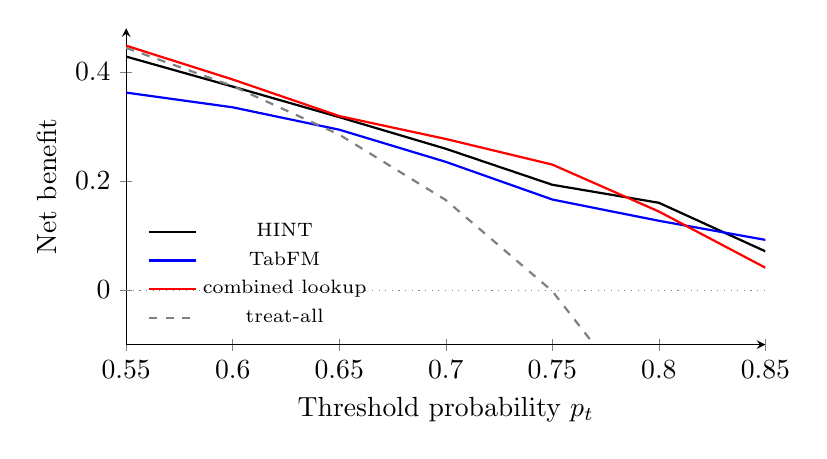
\begin{tikzpicture}
\begin{axis}[
  width=0.8\linewidth, height=5.6cm,
  xmin=0.55, xmax=0.85, ymin=-0.1, ymax=0.48,
  xlabel={Threshold probability $p_t$}, ylabel={Net benefit},
  legend style={font=\scriptsize, at={(0.02,0.02)}, anchor=south west, draw=none, fill=none},
  tick align=outside, axis lines=left, every axis plot/.append style={thick},
]
\addplot[black] coordinates {(0.55,0.428)(0.60,0.373)(0.65,0.317)(0.70,0.259)(0.75,0.193)(0.80,0.160)(0.85,0.071)};
\addplot[blue] coordinates {(0.55,0.362)(0.60,0.335)(0.65,0.294)(0.70,0.235)(0.75,0.166)(0.80,0.127)(0.85,0.092)};
\addplot[red,thick] coordinates {(0.55,0.448)(0.60,0.386)(0.65,0.319)(0.70,0.277)(0.75,0.230)(0.80,0.144)(0.85,0.041)};
\addplot[gray,dashed] coordinates {(0.55,0.444)(0.60,0.374)(0.65,0.285)(0.70,0.165)(0.75,-0.002)(0.80,-0.252)(0.85,-0.670)};
\draw[gray,dotted] (axis cs:0.55,0) -- (axis cs:0.85,0);
\legend{HINT,TabFM,combined lookup,treat-all}
\end{axis}
\end{tikzpicture}
\caption{Decision-curve analysis, phase~III. Above the $0.75$ base rate, treat-all
(dashed) turns harmful and the models add net benefit; but the two-column disease-code$+$drug
base-rate lookup (red) matches or exceeds HINT and TabFM throughout the useful range. Treat-none
is the dotted $y{=}0$ line. \texttt{dca.py}.}
\label{fig:dca}
\end{figure}
\subsection{The metric artefacts that inflate the reported gap}
The reported advantage is largest exactly where the evaluation metric is weakest.
\subsubsection{F1 is uninformative on this benchmark}
\label{sec:f1}
\begin{table*}[t]
\centering
\small
\caption{HINT test F1 under four thresholding rules. Calibration improves F1 but cannot rescue the metric: no rule beats predicting every trial successful.}
\label{tab:f1}
\begin{tabular}{lccc}
\toprule
Decision rule & Phase~I & Phase~II & Phase~III \\
\midrule
Fixed $0.5$ (as published) & 0.5934 & 0.6367 & 0.8123 \\
Validation-calibrated & 0.7125 & 0.6869 & 0.8272 \\
Test-oracle (upper bound) & 0.7119 & 0.7139 & 0.8596 \\
\textsc{Trivial} (all-positive) & \textbf{0.7125} & \textbf{0.7138} & \textbf{0.8569} \\
\emph{positive rate (test)} & \emph{0.553} & \emph{0.555} & \emph{0.750} \\
\bottomrule
\end{tabular}
\begin{minipage}{\linewidth}\vspace{2pt}\scriptsize Source: recomputed from \texttt{preds/preds\_hint\_phase\_\{I,II,III\}.csv} (F1 at each thresholding rule). On phase~I the calibrated and trivial values coincide to four decimals. The oracle sweep ranges over observed scores and therefore excludes the trivial rule, which is why it can fall marginally below it. \end{minipage}
\end{table*}
Calibration helps but cannot rescue the metric (Table~\ref{tab:f1}). Moving from the
published fixed-$0.5$ rule to a validation-calibrated threshold raises HINT's F1 from
$0.593$ to $0.713$ on phase~I and from $0.637$ to $0.687$ on phase~II---gains that look
substantial until compared with the trivial all-positive predictor, which scores $0.713$,
$0.714$ and $0.857$ on the three phases. On phase~I the validation-calibrated F1 equals the
trivial baseline to four decimal places ($0.7125$): the F1-optimal decision rule is to
predict that every trial succeeds. Even the test-oracle threshold---an upper bound that
peeks at the labels---only ties the trivial rule ($0.7139$ vs $0.7138$ on phase~II). When
the best attainable F1 is the one produced by ignoring the input entirely, F1 measures the
class prior, not model quality, and any F1-based ranking on this benchmark is uninformative.
\subsubsection{The claimed advantage tracks metric weakness}
\label{sec:metricweak}
\begin{table*}[t]
\centering
\small
\caption{PR-AUC computed on continuous scores versus on binarised predictions, as HINT\'s evaluation code does. The defect understates PR-AUC in all 15 cells and reorders the variants.}
\label{tab:praucbug}
\begin{tabular}{llccc}
\toprule
 & Variant & PR-AUC (correct) & PR-AUC (binarised) & Error \\
\midrule
Phase~I & Only\_Molecule & 0.6126 & 0.5645 & -0.0481 \\
 & Only\_Disease & 0.6353 & 0.5663 & -0.0690 \\
 & Interaction & 0.6268 & 0.5667 & -0.0601 \\
 & HINT\_nograph & 0.6506 & 0.5781 & -0.0725 \\
 & HINTModel & 0.6443 & 0.5635 & -0.0808 \\
Phase~II & Only\_Molecule & 0.5933 & 0.5735 & -0.0198 \\
 & Only\_Disease & 0.6790 & 0.6166 & -0.0624 \\
 & Interaction & 0.6729 & 0.6097 & -0.0633 \\
 & HINT\_nograph & 0.6724 & 0.6121 & -0.0604 \\
 & HINTModel & 0.6766 & 0.6122 & -0.0644 \\
Phase~III & Only\_Molecule & 0.7800 & 0.7590 & -0.0209 \\
 & Only\_Disease & 0.8647 & 0.8031 & -0.0616 \\
 & Interaction & 0.8588 & 0.8111 & -0.0477 \\
 & HINT\_nograph & 0.8585 & 0.7996 & -0.0589 \\
 & HINTModel & 0.8627 & 0.8154 & -0.0473 \\
\bottomrule
\end{tabular}
\begin{minipage}{\linewidth}\vspace{2pt}\scriptsize Source: recomputed from \texttt{preds/preds\_hintvar\_*\_phase\_\{I,II,III\}.csv} (PR-AUC on continuous scores vs.\ on predictions binarised at $0.5$). Rank agreement between the two computations is $\rho=0.30$ (phase~I), $\rho=0.90$ (phase~II), $\rho=0.70$ (phase~III). On phase~III the bug promotes \texttt{HINTModel} over \texttt{Only\_Disease}. \end{minipage}
\end{table*}
MEXA-CTP's reported gains are largest on PR-AUC (4.1--27.9\%), next on F1 (5.3--19.2\%),
and smallest on ROC-AUC (1.1--3.5\%). These are all \emph{relative} improvements. Read as
\emph{absolute} ROC-AUC differences from MEXA-CTP's own Table~2 --- HINT $0.573/0.621/0.685$
versus MEXA-CTP $0.593/0.638/0.693$ for phases~I/II/III --- the gain is only $+0.020$, $+0.017$
and $+0.008$, i.e.\ $0.008$--$0.020$ ROC-AUC, below the $0.05$ minimum detectable effect of
Section~\ref{sec:power} (Figure~\ref{fig:noisefloor}). We flag the relative/absolute distinction
explicitly because the relative framing makes a sub-noise-floor effect look like a headline
result. The ordering is
also monotone in how badly each metric is computed in the baseline. PR-AUC is understated by
the binarisation defect (Table~\ref{tab:praucbug}); F1 sits below a trivial predictor for both
models (Table~\ref{tab:f1}); ROC-AUC, computed on continuous scores throughout, is the only
sound metric of the three---and it is where the reported gap is smallest and where, under our
protocol, no gap is reproducible at all.
The defect does not merely shift PR-AUC downward; it reorders the models. On phase~III the
best variant under correct computation is the disease-only ablation, but under the binarised
computation it is the full model: the defect promotes the most complex variant over the
simplest.

The clearest symptom that PR-AUC is not comparable across this literature is that the
\emph{same} HINT model, on the \emph{same} phase-III TOP task, is reported at four different
PR-AUC values in four papers (Table~\ref{tab:pracross}): $0.603$ in MEXA-CTP, $0.797$ in
UQ-HINT, $0.811$ in the original HINT paper, and $0.852$ under our continuous-score recomputation
--- a $0.25$ spread on a metric routinely quoted to three decimals. The low outlier ($0.603$)
is the binarised computation; the cluster near $0.80$--$0.85$ is the sound one. A reported
PR-AUC on TOP is therefore uninterpretable without knowing which computation produced it, and
between-paper PR-AUC comparisons are meaningless.

\emph{Three arithmetic tells that the published comparison is unsound.} Beyond the spread, three
facts are checkable with a calculator and each is decisive. \textbf{(a)} MEXA-CTP's reported HINT
PR-AUC of $0.603$ is not merely low --- it is \emph{below the $0.750$ prevalence floor} that even a
random ranker attains on the phase-III test set (positive rate $0.7496$). A model with ROC-AUC
$0.685$ cannot have a PR-AUC beneath the prevalence; $0.603$ is therefore not a valid PR-AUC on this
split but the arithmetic residue of the binarisation bug (D3). \textbf{(b)} MEXA-CTP's own headline
F1 on phase~III, $0.857$, equals the trivial all-positive baseline ($0.8569$) to three decimals: its
best-reported F1 is the score of ignoring the input and predicting ``success'' for every trial
(Section~\ref{sec:f1}). \textbf{(c)} MEXA-CTP's own ablation (its Table~3) reports that token
selection is ``comparable to using all tokens in terms of ROC-AUC,'' and in fact \emph{slightly
worse} than keeping all tokens --- i.e.\ the authors' own numbers already show the mode-experts
token-selection mechanism contributes nothing on the one sound metric, independently corroborating
our finding that the mechanism is inert.
\begin{table}[t]
\centering\small
\caption{The same HINT model, the same phase-III TOP task, four PR-AUC values in four papers.
The $0.603$ outlier is the binarised computation (defect~D3); the $\sim0.80$--$0.85$ cluster is
the sound continuous-score one. Spread $\approx0.25$.}
\label{tab:pracross}
\begin{tabular}{lc}
\toprule
Source (phase~III HINT PR-AUC) & PR-AUC \\
\midrule
MEXA-CTP \citep{zhang2025mexactp} & 0.603 \\
UQ-HINT \citep{chen2024uq} & 0.797 \\
HINT (original) \citep{fu2022hint} & 0.811 \\
This paper (continuous scores) & 0.852 \\
\bottomrule
\end{tabular}
\begin{minipage}{\linewidth}\vspace{2pt}\scriptsize Values transcribed verbatim from each paper's phase-III results table; our value from \texttt{preds/preds\_hint\_phase\_III.csv} on continuous scores. (LINT is excluded: it reports a different, non-phase-split approval task.) \end{minipage}
\end{table}
We do not suggest the MEXA-CTP authors computed the baseline incorrectly. They inherited the
baseline's own evaluation code, which is precisely the point: \textbf{a defect in a reference
model's evaluation propagates into every comparison made against it}. HINT is the reference model for this benchmark and the base of downstream work \citep{chen2024uq}, so the propagation surface is wide. We flag this as a risk to be audited, not as a finding we have verified beyond the case examined here.
% =====================================================================
\subsection{The limit of measurability}
Finally, we bound what any comparison on this benchmark can establish at its current size.
\subsubsection{Statistical power: phase-III differences below $0.05$ ROC-AUC are unverifiable}
\label{sec:power}
The comparisons above should be read through what the benchmark can actually resolve. We make
this quantitative on phase~III (\texttt{stats\_rigor.py}).

\emph{Differences of AUCs, with DeLong.} Per-model CIs (Tables~\ref{tab:fair},
\ref{tab:baselines}, \ref{tab:ablation}, \ref{tab:gbdt}) and their visual overlap
(Figure~\ref{fig:forest}) do not test a \emph{difference}; two CIs can overlap while the
paired difference is significant, and vice versa. For correlated AUCs the DeLong test does test
it, more cheaply than bootstrap, and we use it in place of any overlap argument. On phase~III:
HINT$-$TabFM $=+0.018$ (SE $0.018$, $95\%$ CI $[-0.017,+0.053]$, $p=0.33$); HINT$-$GradBoost
$=+0.034$ (SE $0.018$, $95\%$ CI $[-0.000,+0.068]$, $p=0.052$); HINT$-$(disease-code base rate)
$=-0.009$ ($95\%$ CI $[-0.036,+0.018]$, $p=0.52$). None reaches significance --- HINT vs
gradient boosting only marginally so --- so no model, deep or tabular, is shown to beat another.

\emph{Non-parametric confirmation.} The null results are not an artefact of DeLong's normal
approximation. A paired sign-flip \emph{permutation} test (2{,}000 resamples, swapping HINT and
TabFM per-trial scores) reproduces the HINT$-$TabFM result exactly ($p=0.34$ vs DeLong's
$0.33$). On the A/B cross-attention arms, a Wilcoxon signed-rank test over the seven matched
phase-III pairs gives $p=0.81$ (paired $t$ gave $0.96$), so ``training the cross-attention does
nothing'' survives a distribution-free test too. Finally, the validation-selected F1 threshold
is stable under resampling: bootstrapping the validation set (1{,}000 resamples) and re-selecting
the F1-optimal threshold gives a threshold of $0.44\pm0.04$ and a resulting test F1 of
$0.829\pm0.014$ ($95\%$ CI $[0.814,0.851]$) --- always below the trivial all-positive $0.857$.
The metric conclusions do not depend on the choice of test or on a single lucky threshold.

\emph{But ``not significant'' is not ``equivalent.''} A two one-sided tests (TOST) procedure at
an equivalence margin $\delta=0.02$ does \emph{not} establish
equivalence for HINT vs TabFM ($p=0.45$): the data are consistent both with no difference and
with a difference up to $\sim$0.05. We set $\delta=0.02$ on two aligned grounds: it is on the scale
of the benchmark's test-sampling standard error for a between-model difference ($\approx0.018$; a
``difference'' smaller than the noise on which it is measured is not meaningfully a difference), and
it is clinically negligible --- at the phase-III base rate a $0.02$ ROC-AUC shift moves essentially
no go/no-go decision and is dwarfed by the label noise of a manually curated outcome
(Section~\ref{sec:intro}); a margin this small makes the equivalence test \emph{harder} to pass, so
failing it is a statement about power, not a lax threshold. We therefore avoid the word ``equivalent'' and state the
weaker, correct claim: no difference is \emph{detectable}, because the study is underpowered.
Throughout the paper, where we call two models ``indistinguishable'' we mean precisely this ---
no difference detectable at this sample size, i.e.\ below the minimum detectable effect derived
next --- not demonstrated equivalence.

\emph{The minimum detectable effect, per phase.} With $n{=}1146$ predictions the DeLong standard
error of $\Delta$AUC is $0.018$, so the smallest difference detectable at $80\%$ power and
$\alpha{=}0.05$ is $\mathbf{0.05}$ ROC-AUC on phase~III. The MDE is phase-specific, scaling with
each split's size: from the same computation it is $\approx0.067$ on phase~I ($n{=}627$),
$\approx0.035$ on phase~II ($n{=}1654$) and $\approx0.050$ on phase~III ($n{=}1146$). \textbf{On
every phase, any claimed between-model gain below its MDE ($0.035$--$0.067$) is unverifiable at
this sample size} --- and every gain reported in this literature, and every gain we ourselves
ever formed, is below it.
The number is correlation-dependent: the DeLong SE shrinks as the two models' predictions
agree, so $0.05$ is the MDE for a pair as correlated as HINT and TabFM; a pair that agreed less
would need an even larger effect to detect, never a smaller one, so $0.05$ is a floor on the
MDE, not a worst case. The A/B comparison of Table~\ref{tab:ab} has its own, larger MDE: seven
matched pairs with a paired-difference sd of $0.020$ can detect only $|\Delta|>0.025$ at $80\%$
power, against an observed $+0.0004$ --- so ``training the cross-attention does nothing'' is
also, in part, a statement about power. This is the quantitative form of the paper's thesis
(Figure~\ref{fig:noisefloor}).
\begin{figure}[htbp]
\centering
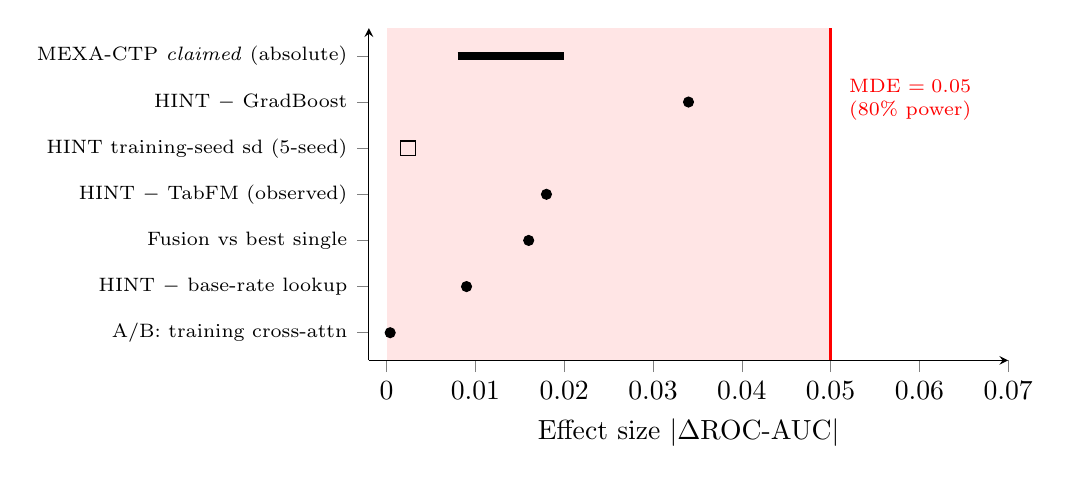
\begin{tikzpicture}
\begin{axis}[
  width=0.8\linewidth, height=5.8cm,
  xmin=-0.002, xmax=0.07,
  xlabel={Effect size $|\Delta\text{ROC-AUC}|$},
  scaled x ticks=false,
  x tick label style={/pgf/number format/fixed, /pgf/number format/precision=2},
  ytick={0,1,2,3,4,5,6},
  yticklabels={{A/B: training cross-attn},{HINT $-$ base-rate lookup},{Fusion vs best single},{HINT $-$ TabFM (observed)},{HINT training-seed sd (5-seed)},{HINT $-$ GradBoost},{MEXA-CTP \emph{claimed} (absolute)}},
  y tick label style={font=\scriptsize}, ymin=-0.6, ymax=6.6,
  axis lines=left, tick align=outside, enlarge y limits=false,
]
\fill[red!10] (axis cs:0,-0.6) rectangle (axis cs:0.05,6.6);
\draw[red,thick] (axis cs:0.05,-0.6) -- (axis cs:0.05,6.6);
\node[red,anchor=south west,font=\scriptsize,align=left] at (axis cs:0.051,4.4){MDE $=0.05$\\(80\% power)};
\addplot[only marks,mark=*,black,mark size=1.8pt]
  coordinates {(0.0004,0) (0.009,1) (0.016,2) (0.018,3) (0.034,5)};
\addplot[only marks,mark=square,black,mark size=2.6pt]
  coordinates {(0.0024,4)};
\draw[black,line width=3pt] (axis cs:0.008,6) -- (axis cs:0.020,6);
\end{axis}
\end{tikzpicture}
\caption{Every effect we observe or that the literature claims sits at or below the minimum
detectable effect (MDE $=0.05$ ROC-AUC at $80\%$ power, $n{=}1146$; shaded). The axis is
\emph{absolute} $\Delta$ROC-AUC. Crucially, MEXA-CTP's headline ``$1.1$--$3.5\%$'' is a
\emph{relative} improvement over HINT; read as absolute ROC-AUC differences from MEXA-CTP's own
Table~2 they are only $+0.020$, $+0.017$ and $+0.008$ for phases~I, II and~III (bar spans
$0.008$--$0.020$) --- about half what the percentage suggests, and entirely inside the shaded
region. Our fusion and between-model differences, and even HINT's advantage over gradient
boosting, likewise all fall where a difference cannot be verified at this benchmark's phase-III
size. The ``HINT training-seed sd'' point is drawn as an open square ($\square$) to mark that it is
a \emph{standard deviation} (a genuine $5$-seed retraining sd, $0.0024$; Section~\ref{sec:power}),
not an effect-size estimate like the filled circles --- HINT is reproducible across seeds, and the
noise that swamps between-model effects is test-set sampling, not seed.}
\label{fig:noisefloor}
\end{figure}

\emph{This is ``differences unmeasurable,'' not ``nothing works.''} The models do carry real,
if shallow, signal, and the ranking metrics understate it: HINT reaches balanced accuracy
$0.63$ and Matthews correlation $+0.27$ (TabFM $0.53$ / $+0.12$), and PR-AUC sits $+0.10$ above
the $0.75$ prevalence floor ($0.852$ vs $0.750$). The finding is precise --- \emph{the models
cannot be told apart from each other or from a disease-code base rate} --- not the stronger and
false ``the task is unlearnable.'' (The threshold-metric gap, HINT's balanced accuracy $0.63$
vs TabFM's $0.53$, also shows that ranking-tied models can differ once a decision is made,
echoing the calibration result of Section~\ref{sec:calibration}.)

\emph{Where the variance comes from.} The three uncertainty sources that Table~\ref{tab:reload}
warned against conflating separate as: test-resampling (bootstrap/DeLong SE $\approx0.018$ on
$\Delta$AUC), training-seed (TabFM $32$-member sd $0.0011$ over five seeds; for HINT we now
\emph{measure} it by retraining five times, seeds $2023$--$2027$: test ROC-AUC $0.685\pm0.0024$,
range $[0.682,0.687]$ --- only about twice TabFM's and, importantly, an order of magnitude
\emph{below} the test-resampling SE that sets the MDE), and split variance (a single temporal
split; as an \emph{indicative} probe we re-score on time-ordered sub-windows of the test set,
where the lookup and HINT vary with sd $\approx0.02$--$0.04$. This is only a gauge, not a clean
estimate: each window has a fraction of the trials, so its variance is inflated by within-window
\emph{sampling} noise and cannot be read as the split term alone --- a proper estimate would
re-derive train/test at several cut dates, which we leave to future work). The single $n{=}2$ difference of
$0.023$ we reported earlier (run~A vs run~B, Table~\ref{tab:ablation}) additionally reinitialised
the encoders and is an outlier against this five-seed sd; we correct the record here. The
takeaway is unchanged and in fact firmer: HINT's training-seed variance is small, so the noise
that swamps between-model effects is \emph{test-set sampling} ($0.018$), not seed. We also check that TabFM's near-zero seed variance is not an
ensembling artefact: a \emph{single}-member TabFM ($n_{\text{est}}{=}1$) is exactly
deterministic across five seeds (phase-III ROC-AUC $0.668$, sd $0.0000$), so the $32$-member
sd of $0.0011$ is if anything slightly \emph{larger}, coming from subsample randomness --- the
foundation model's reproducibility is intrinsic, not bought by averaging. Test-resampling alone
already puts the MDE at $0.05$; adding seed and split variance can only raise it.

\emph{Multiplicity policy: primary versus secondary contrasts.} We state this
once and apply it throughout, because the correction a contrast receives should follow from its
role, not from whether it happened to reach significance. This is a retrospective re-analysis, so
we say \emph{primary} and \emph{secondary} rather than ``pre-registered''; the primary contrasts
are the few hypothesis-testing comparisons that carry the paper's claims, and they
are the only ones we correct or hold to $\alpha{=}0.05$: (i) the three primary between-model
DeLong tests on phase~III (HINT vs TabFM, vs tuned gradient boosting, vs the disease-code base
rate, Section~\ref{sec:power}); and (ii) the phase-III fusion family, where we deliberately
searched $4\times3\times2=24$ combiner/member/metric contrasts for a win and therefore report
Benjamini-Hochberg FDR and Bonferroni over the whole family (Table~\ref{tab:fusioncorr}).
Everything else is \textbf{exploratory} and labelled as such: the $7{\times}11$ model$\times$feature
grid (Section~\ref{sec:tabfm}) is selected on \emph{validation} with a single test touch, so it
is a selection procedure, not a test family; the per-ICD-chapter strata
(Table~\ref{tab:complement}) and the PR-AUC binarisation table (Table~\ref{tab:praucbug}) are
descriptive; the A/B cross-attention comparison (Table~\ref{tab:ab}) is powered only on
phase~III and reported per phase. We do not pool across phases (different prevalences, sizes and
effects --- not exchangeable), which is why we dropped the earlier cross-phase $t$-test. No
exploratory contrast is used to assert a positive finding; where one is significant before
correction (the three phase-III fusion edges) it does not survive the confirmatory family, and
we report it as not surviving. Bootstrap CIs use unstratified resampling; this is immaterial
not only at phase~III ($n{=}1146$, $0.75$ prevalence) but also at the smaller, more balanced
phase~I ($n{=}627$, $0.55$), where stratified and unstratified HINT CIs coincide
($[0.525,0.619]$ vs $[0.528,0.618]$). DeLong is the primary inferential tool. Where we test a
between-model difference we also report a paired sign-flip \emph{permutation} test --- a
distribution-free alternative that makes no normality assumption on correlated AUCs --- and it
reproduces DeLong throughout (HINT$-$TabFM $p=0.34$ vs $0.33$).
% =====================================================================
\section{What we got wrong, and what fixed it}
\label{sec:wrong}
This section is evidence, not an appendix. Seven directional findings were formed during this
work; under tightened methodology six were overturned and the remaining one --- the PR-AUC bug ---
narrowed to a single phase rather than dissolving outright (Table~\ref{tab:dissolved}).
Their consistency is the result.
\begin{table*}[t]
\centering
\small
\caption{Seven directional findings formed during this work, and what happened to each when the methodology was tightened: six were overturned, one (the PR-AUC bug) narrowed. Their consistency is the central result.}
\label{tab:dissolved}
\begin{tabular}{p{3.4cm}p{2.6cm}p{2.6cm}p{2.8cm}}
\toprule
Claim as first formed & Original basis & Tightening & Outcome \\
\midrule
Routing is harmful ($\tau{=}0$ helps) & 1 seed, $+0.019$ & 3 seeds & $+0.002$; dissolved \\
Training attention slightly hurts & 9 pairs, $p\approx0.056$ & 12 pairs, 7 seeds on III & $p=0.229$; dissolved \\
PR-AUC bug flatters complex models & phase~III only & phases~I, II added & holds on III only; narrowed \\
22 binary features match the deep model & best of 12, chosen on \emph{test} & chosen on \emph{validation} & reverses: HINT $+0.009$ \\
Tabular model beats HINT & best cell on \emph{test} & best cell on \emph{validation} & equivalent (Table~\ref{tab:tabfm}) \\
Blending members gives a medium gain & fusion $>$TabFM, $+0.034$ ROC on III & vs best single; 24-contrast FDR sweep & $+0.016$ vs HINT; 0 survive; dissolved \\
Seed noise ($\sim$0.02--0.03) swamps all effects & $n{=}2$ run-to-run $0.023$ & five-seed retraining & sd $0.0024$; dissolved --- test-sampling, not seed, is the floor \\
\bottomrule
\end{tabular}
\begin{minipage}{\linewidth}\vspace{2pt}\scriptsize Source: Section~\ref{sec:wrong}; current values in \texttt{ab\_test\_results\_phase\_*.csv}, \texttt{preds/preds\_hintvar\_*.csv}, \texttt{icd\_representation\_phase\_*.csv}, \texttt{tabular\_grid\_phase\_*.csv}, \texttt{optionB\_phaseIII\_multiplecomparison.csv}. \end{minipage}
\end{table*}
The first illustrates a specific statistical error worth naming. The effect was judged real
because it appeared to be many standard deviations from zero---but the standard deviation
had been estimated from a \emph{different} MEXA-CTP routing configuration ($\tau=0.3$, seed sd
$0.0024$ --- a coincidence of value with, but unrelated to, HINT's five-seed sd above) than
the one under test ($\tau=0.0$, seed sd $0.0221$, roughly ten times larger). Noise must be
estimated per configuration.
The fourth is the sharpest. Selecting the best of twelve pipelines by test score is exactly
the error this paper criticises in MEXA-CTP's epoch selection. We reproduced the flaw we set
out to document, in our own re-analysis, and caught it only by imposing on ourselves the
discipline we demanded of others. The same trap reappeared in the larger $7\times11$ tabular
grid of Section~\ref{sec:tabfm}: ranked by test score the grid appears to \emph{beat} HINT in
phases~I and~II, but the validation-selected winner is merely \emph{equivalent}---the naive
reading was again an artefact of selecting on test (the \emph{Tabular model beats HINT} row of Table~\ref{tab:dissolved}).
\paragraph{Errors in the re-analysis code.} Two further defects were caught by controls
rather than by crashes. Run directories collide across phases, so phase~I outputs silently
overwrote phase~III's. And ICD features were read in dataset order while labels were read in
CSV order, misaligning rows and collapsing ROC-AUC to near chance---a result that, had it not
been checked against an independent control, would have supported a dramatic and entirely
false claim.
\paragraph{Errors at drafting.} Twice, numbers drifted between analysis and prose. Arm means
were transcribed from an earlier three-seed run into a table labelled seven-seed. More
seriously, we recorded MEXA-CTP's headline claim as ``4.9\%''---a figure that appears nowhere
in that paper. A paper arguing that others reported numbers carelessly cannot itself misquote
the number it contests. Correcting it produced Section~\ref{sec:metricweak}: the misquote had
collapsed three metrics into one figure and destroyed the structure carrying our strongest
argument. Every table in this paper is generated from stored predictions by script; every
figure quoted from another paper is traced to a verbatim sentence in it.
\medskip
\noindent\textbf{Implication.} Every one of these errors produced a plausible,
publishable-looking result. None crashed. None was visible without deliberate replication. On
a benchmark where true effect sizes are around $0.01$ ROC-AUC and the sampling noise on a
between-model difference is $\approx0.018$ (an order of magnitude above either model's
training-seed sd), this is the expected failure mode, not an unusual one.
% =====================================================================
\section{Limitations}
\begin{itemize}\itemsep2pt
  \item \textbf{Statistical power.} After matching and de-duplication the A/B comparison
        rests on 7 pairs (phase~III), 3 (phase~II) and only 2 (phase~I). Phase~I is
        uninformative rather than weakly suggestive.
  \item \textbf{Known high-signal metadata is absent from the processed data.} Enrollment
        count, sponsor type and trial start year are strong, standard predictors, but the TOP
        CSVs shipped with HINT contain only \texttt{nctid, status, why\_stop, label, phase,
        diseases, icdcodes, drugs, smiless, criteria} --- none of the three. Recovering them
        requires re-deriving from the raw ClinicalTrials.gov XML (the benchmark's
        sponsor-inference pipeline does this for sponsor). All tabular models here, ours and
        the GBDTs, are therefore evaluated without these features; adding them is the most
        promising next step and could raise every tabular baseline. We state the direction
        explicitly, since it is easy to read as a threat: if these features lift the tabular
        baselines, they \emph{strengthen} the paper's thesis rather than weaken it --- simple
        per-trial features would beat the deep models by even more, and the deep architecture's
        marginal contribution over cheap tabular signal would remain unmeasurable. There is no
        configuration of this experiment in which richer metadata rescues the deep models.
  \item \textbf{HINT's training-seed sd, now measured.} We retrained HINT five times (seeds
        $2023$--$2027$) on phase~III: test ROC-AUC $0.685\pm0.0024$ (range $[0.682,0.687]$). HINT
        is therefore reproducible across training seeds --- its seed sd ($0.0024$) is about twice
        TabFM's ($0.0011$) and an order of magnitude below the test-resampling SE ($0.018$) that
        sets the MDE. This supersedes the single $n{=}2$ difference of $0.023$ we first reported
        (run~A vs run~B), which reinitialised the encoders and was an outlier; no conclusion
        rested on it, and the corrected, smaller sd only firms the power argument. The one term we
        do not cleanly isolate is split variance (a single temporal split); our sub-window gauge
        (Section~\ref{sec:power}) puts it at sd $\approx0.02$--$0.04$ but is confounded with
        per-window sampling noise, so a multi-cut re-split is the proper measurement, left to future work.
  \item \textbf{Baseline features.} Classical baselines use MEXA-CTP's embeddings, not
        HINT's own encoders. A fully matched comparison would also run gradient boosting on
        HINT's features.
  \item \textbf{The tabular baseline uses different features from HINT's encoders.} The
        zero-training baseline (Section~\ref{sec:tabfm}) uses interpretable RDKit/ICD/protocol
        features, not HINT's learned embeddings; the two constructions agree, but neither is a
        byte-for-byte match of HINT's inputs. The GRAM feature set also exceeds the foundation
        model's feature cap, so its winning result is carried by classical learners.
  \item \textbf{HINT's criteria modality is dead under the shipped cache (D5) --- now measured,
        and inert.} Because \texttt{sentence2embedding.pkl} is empty, every HINT run here (and in
        the public repository) feeds a zero vector to the eligibility-criteria branch. We
        regenerated the full BioBERT cache and re-scored HINT with a live branch
        (Section~\ref{sec:defects}): the effect on phase-III performance is $\Delta$ROC-AUC
        $=-0.0001$ ($p=0.93$) and $\Delta$PR-AUC $=+0.0002$ ($p=0.78$) --- a real defect with no
        measurable effect on HINT's numbers. The one check still owed is a full
        \emph{retrain}-from-scratch with the live cache (blocked here by defect~D10); we do not
        expect it to change the verdict, since re-scoring the trained model with real criteria
        embeddings already changes nothing. We therefore still make no claim that
        eligibility-criteria \emph{text} is uninformative in general --- only that HINT does not
        use it.
  \item \textbf{The fusion gain is single-checkpoint.} The phase-III HINT+TabFM gain varies
        the tabular model's seed against one fixed HINT checkpoint; a fuller estimate would
        vary HINT's training seed as well, and the per-area strata behind it hold only
        40--140 trials each (Table~\ref{tab:complement}).
  \item \textbf{The full-masking guard modifies the architecture.} Retaining one unmasked
        token is minimal and intent-preserving, but it is a modification; it is applied to
        both arms.
  \item \textbf{Distribution shift between splits.} Validation and test positive rates differ
        (Table~\ref{tab:splits}), so validation-selected thresholds underperform test-oracle
        thresholds. The protocol is correct; the shift should be reported.
  \item \textbf{Anachronistic disease coding.} Our tabular front-end encodes trials with the
        2024 ICD-10-CM hierarchy, but the trials predate it (train completed before 2014). Using a
        coding version that postdates the trials is a mild anachronism shared by any modern
        re-encoding; it affects all tabular models equally and cannot manufacture a between-model
        difference, but a period-correct ontology would be cleaner.
  \item \textbf{The benchmark's base rate is not the field's.} TOP's phase-III positive rate is
        $0.75$, well above the $\sim$55--60\% phase-III-to-approval likelihood reported in the
        industry literature \citep{hay2014clinical,wong2019estimation}. This gap --- consistent with
        the label mixing (``endpoint met'' vs ``drug progressed'') and curation selection we flag in
        Section~\ref{sec:dataquality} --- means the benchmark is easier than the real decision and
        caps the external validity of any TOP result, ours included.
  \item \textbf{We address protocol, not contamination.} Our protocol does not establish that
        a trial's outcome was unknown at prediction time. CT~Open \citep{wang2025ctopen} shows
        this is a real and separate threat; both checks are necessary.
  \item \textbf{Propagation is hypothesised, not measured.} We verified the PR-AUC defect in
        HINT's code and observed its effect on the MEXA-CTP comparison. We did not audit
        downstream work and make no claim about it.
\end{itemize}
% =====================================================================
\section{Conclusion}
Under a shared, corrected protocol, the reported advantage of MEXA-CTP over HINT does not
survive; no difference between the two is detectable (below a minimum detectable effect of
$\approx0.05$ ROC-AUC at this sample size, Section~\ref{sec:power}), and neither clearly beats gradient boosting on the
same inputs. MEXA-CTP's central mechanism was never trained in the released artifact, and
once repaired contributes nothing measurable. HINT's multimodal architecture contributes
nothing measurable over its disease codes alone. A zero-training tabular foundation model,
and indeed any of a broad panel of classical learners once selected on validation, matches
HINT in every phase using disease-ontology features alone, at zero training cost and with
comparable seed reproducibility (TabFM sd $0.0011$, HINT $0.0024$ over five retrainings).
Combining models yields no gain over the best single model
once the choice of combiner and metric is corrected for: the small phase-III edge exists only
against the weaker member and does not survive multiple-comparison correction, so it is not
evidence for the deep interaction mechanism.
The broader result is that claimed effect sizes on this benchmark lie below measurement
noise. We demonstrate this not only by measuring the noise but by documenting seven of our own directional findings that did not survive replication. Improvement claims on TOP should be accompanied by multiple seeds, validation-based selection of every free choice, confidence intervals, and a trivial baseline---or they are not verifiable.
Two directions follow. In the short term, a shared evaluation harness costs little and should accompany any benchmark whose reference implementation is reused as a baseline, since a defect in that implementation's evaluation code silently biases every subsequent comparison. In the longer term, retrospective benchmarks may not be repairable by protocol alone: CT~Open \citep{wang2025ctopen} argues that contamination is a second, independent failure mode, and its live time-stamped design removes both at once. We regard that as the right destination; the contribution of this paper is to show how much of the existing retrospective literature does not survive the first of the two checks.
\paragraph{What a $0.70$-ROC model could actually do.} It is worth being concrete about the
clinical stakes, since accuracy is not benefit \citep{fritz2024effect}. At ROC-AUC $\approx0.70$
and the $0.75$ base rate of phase~III, a model cannot safely gate a go/no-go decision: at any
threshold that flags a useful fraction of failures it also discards many eventual successes,
and the F1-optimal rule is still ``predict every trial succeeds'' (Table~\ref{tab:f1}). The
realistic use is triage, not decision --- ranking a portfolio so that the lowest-scoring, say,
$10\%$ receive extra scrutiny --- and even there a per-indication historical base rate
(Section~\ref{sec:dataquality}) would rank almost identically, so the model earns its keep only
if it beats that lookup, which on TOP it does not. The ORACLE trial \citep{fritz2024effect} is
the cautionary precedent: a model that raised agreement without raising accuracy. Any
deployment claim on this benchmark should therefore state the decision, the threshold, and the
base-rate baseline it must beat --- none of which a headline ROC number supplies.
\paragraph{Responsible disclosure.} We frame every code-level defect in this paper (D1--D10,
including the un-trained mode-experts mechanism, the empty eligibility-criteria cache, and the
binarised PR-AUC computation) as an ecosystem reproducibility hazard, not as author misconduct.
Each is reproducible from the unmodified public repositories, and several --- the empty cache
and the released-checkpoint reload variance in particular --- silently affect anyone who
re-runs the code, which is precisely why they matter. Following responsible-disclosure
practice, we reported the defects to the respective project maintainers through their public
issue trackers before submission: HINT issue \#15
(\url{https://github.com/futianfan/clinical-trial-outcome-prediction/issues/15}; audited commit
\texttt{8dc0497}) and MEXA-CTP issue \#2 (\url{https://github.com/murai-lab/MEXA-CTP/issues/2};
audited commit \texttt{b898dbb}), both also recorded in \texttt{DISCLOSURE.md} with the code
release. Our aim is to harden a shared
benchmark that the whole subfield depends on, and we would welcome corrections from the original
authors.
\paragraph{Reproducibility.} All code, raw per-trial predictions and result tables are released at \url{https://github.com/azizcetinerr/top-benchmark-reeval}. All defect audits are time-stamped: the HINT repository was audited at commit \texttt{8dc0497} and MEXA-CTP at commit \texttt{b898dbb} (both July 2026; full hashes in \texttt{DISCLOSURE.md}). Every table in this paper is regenerated from stored predictions without retraining. Settings: seed 2023, ICD-10-CM 2024, BioBERT \texttt{dmis-lab/biobert-v1.1}, 1000 bootstrap resamples at 95\% for all confidence intervals and paired tests, except the phase-III multiple-comparison stress test (Section~\ref{sec:optionb}), which uses 10{,}000 resamples to stabilise the corrected $p$-values. The tabular baselines of Section~\ref{sec:tabfm} additionally use TabFM (\texttt{tabfm-1.0.0-jax}) with $32$ ensemble members and RDKit 2026.03 for molecular descriptors and Morgan fingerprints. Feature construction: RDKit descriptors are aggregated across a trial's drugs by mean and max; Morgan/ECFP fingerprints use radius $2$ and $256$ bits, combined across drugs by bit-union (a bit is set if present in any drug); GRAM disease features are multi-hot over ontology ancestors. The tuned gradient-boosting baselines (Section~\ref{sec:gbdt}) use XGBoost 3.2, LightGBM 4.7 and CatBoost 1.2, each grid-selected on validation.
%\bibliographystyle{model1-num-names}
\bibliographystyle{cas-model2-names}
\bibliography{cas-refs}
% Biography
%\bio{}
% Here goes the biography details.
%\endbio
%\bio{pic1}
% Here goes the biography details.
%\endbio
\end{document}
